
\chapter{Introduction au séquençage par translocation à travers un pore}
\label{intro}

\cleardoublepage

{\Large\textbf{{Introduction au séquençage par translocation à travers un pore}}}\\


\lettrine[loversize=0.6,lraise=0.1,findent=0.5em,nindent=0em]{D}{}ans ce chapitre nous introduisons les notions et  concepts nécessaires à la compréhension du séquençage par translocation à travers un nanopore. L'aspect expérimental est abordé dans un premier temps à travers l'ADN et l'historique de son séquençage, puis les différentes utilisations des nanopores et les techniques de mesure de courant de translocation visant à établir la séquence de la biomolécule en translocation. Une introduction br\^eve des modèles théoriques de l'étude de la translocation sera suivie par un inventaire des différentes modélisations numériques.

\minitoc

\begin{center}
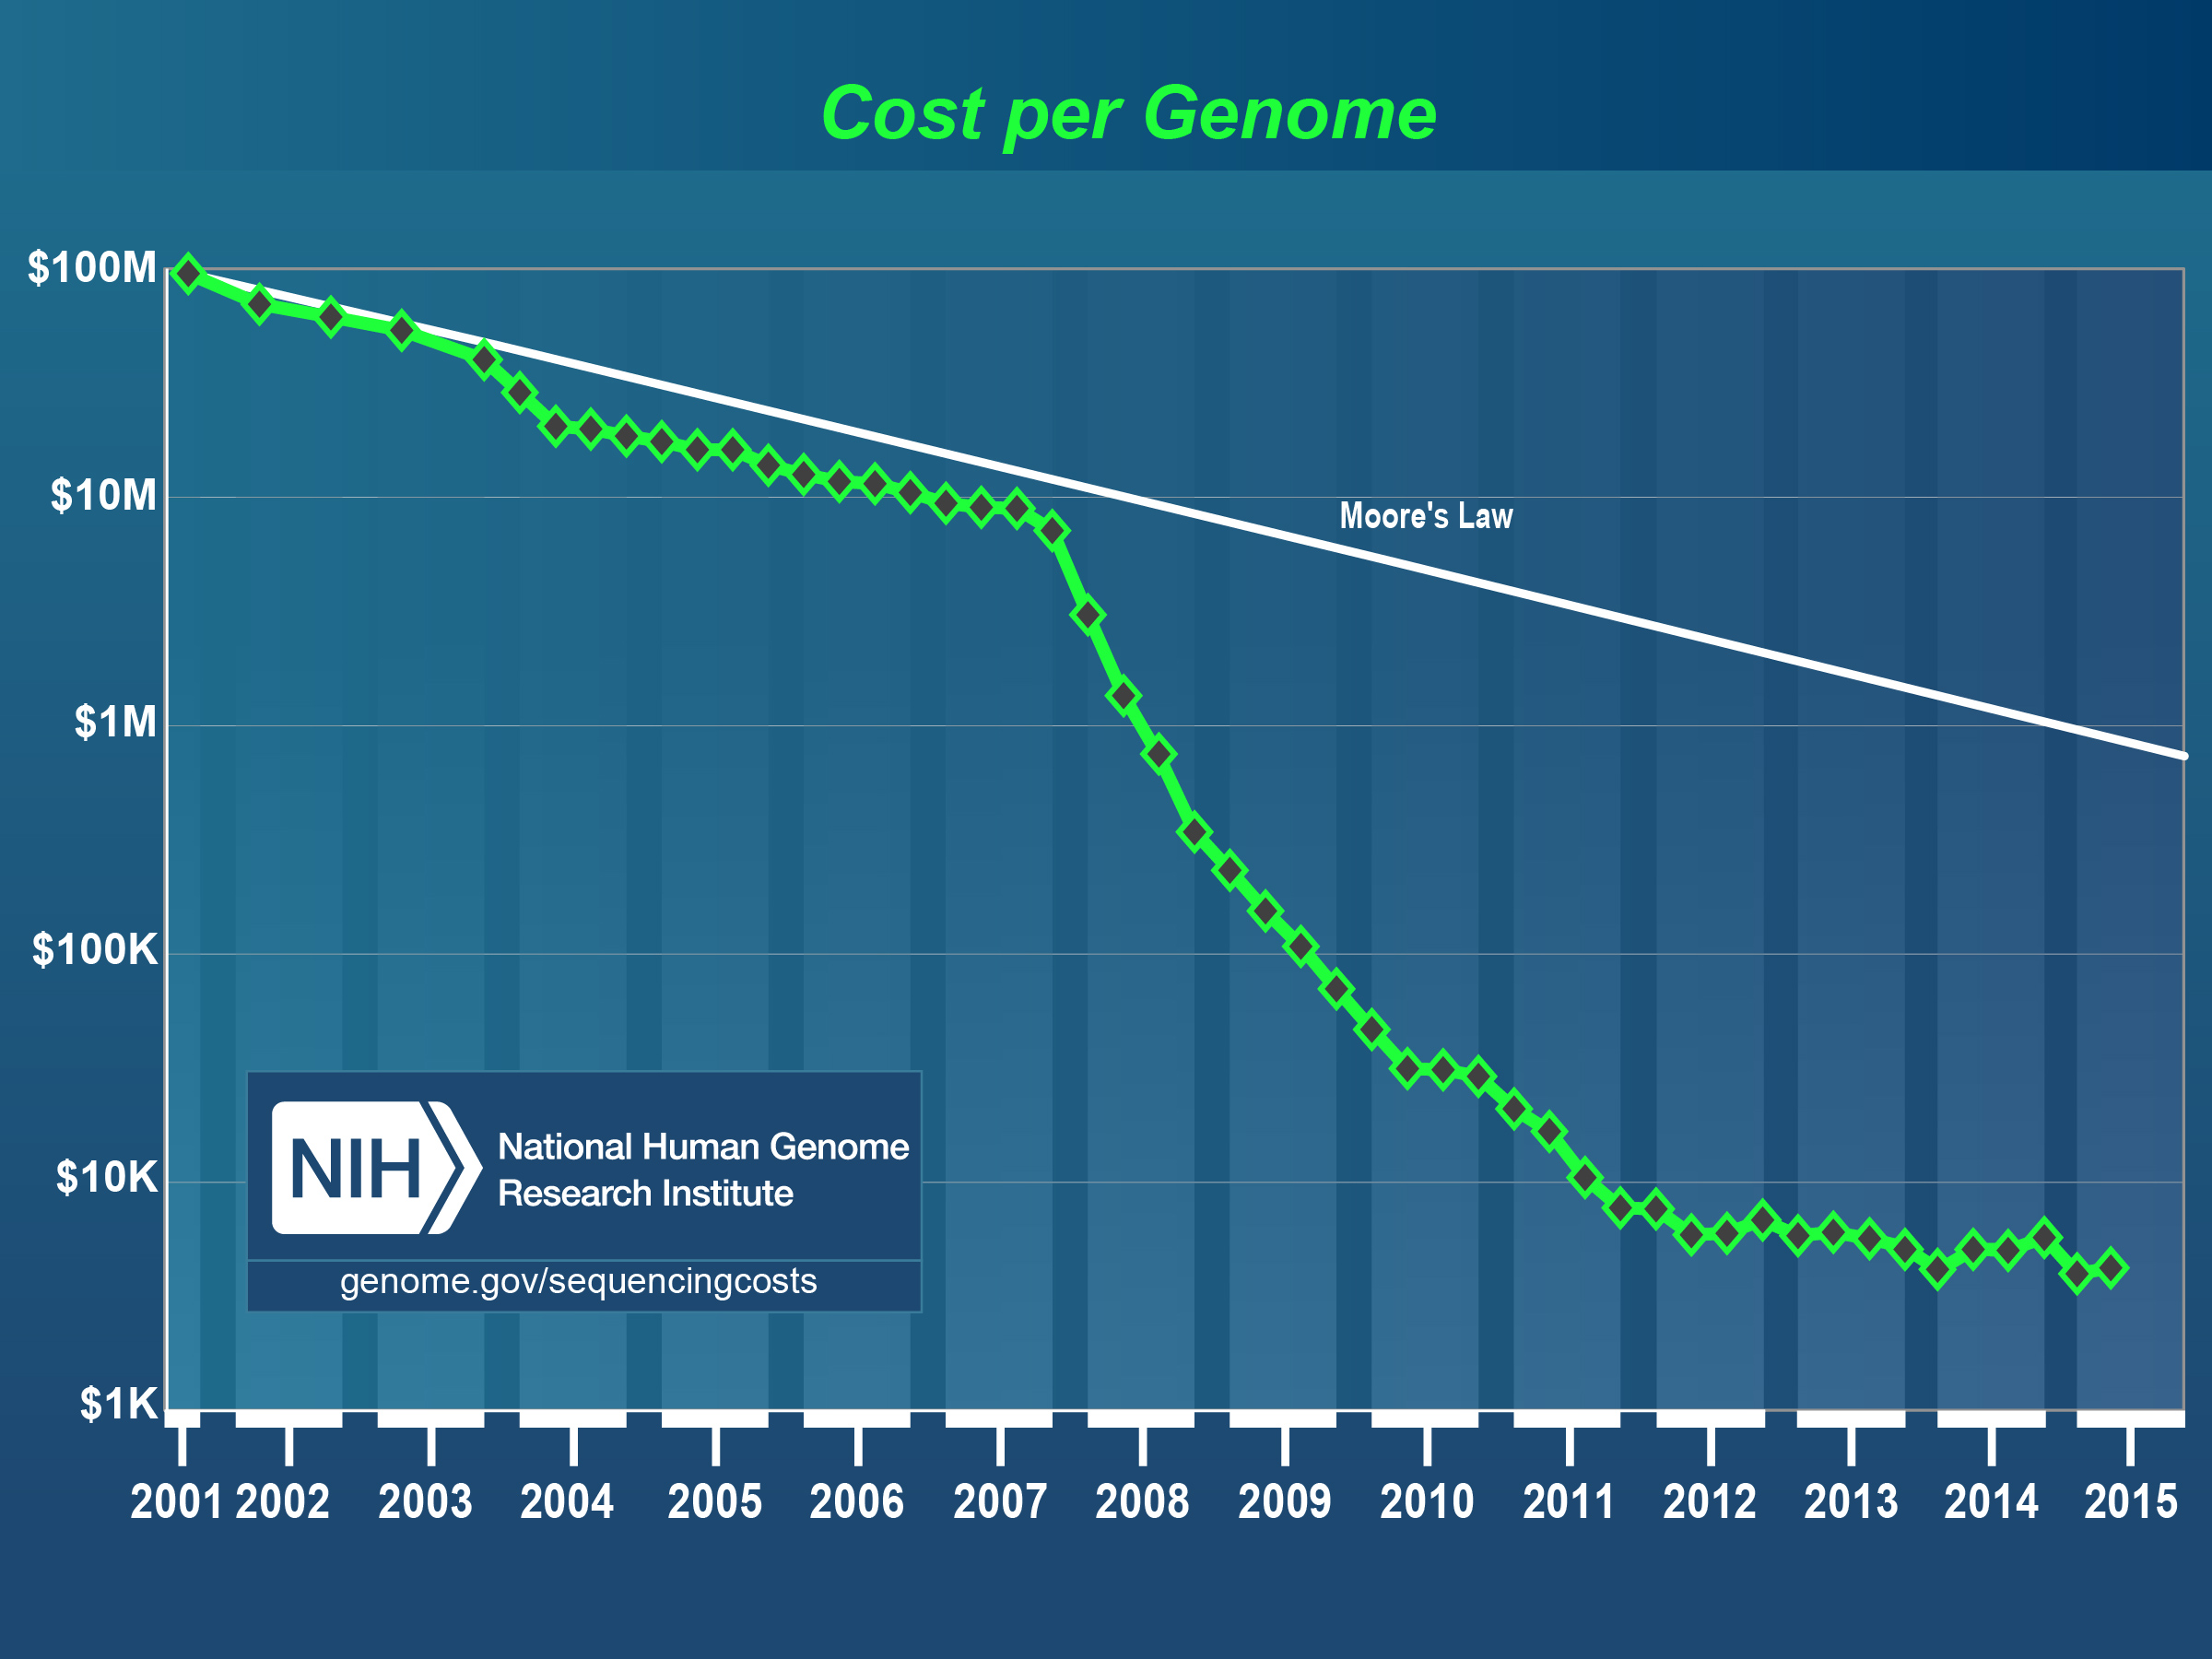
\includegraphics[width=0.7\textwidth]{cost_genome.jpg}
\end{center}





\cleardoublepage




\section{Contexte technologique}

\subsection{L'ADN et le séquençage}

Les bio-polymères, et notamment l'ADN (Acide DésoxyriboNucléique), sont les polymères qui constituent le vivant. Ils interviennent dans de nombreux processus clés en biologie.  L'ADN, avec l'ARN (Acide RiboNucléique) est le support de l'information génétique du vivant. \\

L'ADN, généralement contenu dans le noyau des cellules, a été pour la première fois isolé et identifié par Friedrich Miescher en 1869 à partir de globules blancs. En 1953, Francis Crick et James Watson mettent en évidence sa fameuse structure en double hélice \cite{watsoncrick}. Cette hélice est le reflet de la conformation dite double brin de l'ADN, il s'agit de l'appariement de deux chaînes dites simple brin qui sont complémentaires. Le simple brin d'ADN est une séquence de quatre monomères différents. Ces monomères, appelés nucléotides sont constitués de phosphate, de sucre et d'une des bases azotées, seul élément distinct entre nucléotides: l'adénine, la guanine (deux purines), ainsi que la cytosine et la thymine (deux pyridines). Via des liaisons hydrogènes (aussi appelée liaisons Watson-Crick dans le cas de l'ADN), les bases peuvent s'associer à leur complémentaire, adénine avec thymine et cytosine avec guanine. Les liaisons hydrogènes favorisent une forte affinité lors de l'appariement et contribuent avec les interactions orbitalaires entre cycles aromatiques des bases azotées à stabiliser cette structure hélicoïdale.

\begin{figure}[H]
\begin{center}
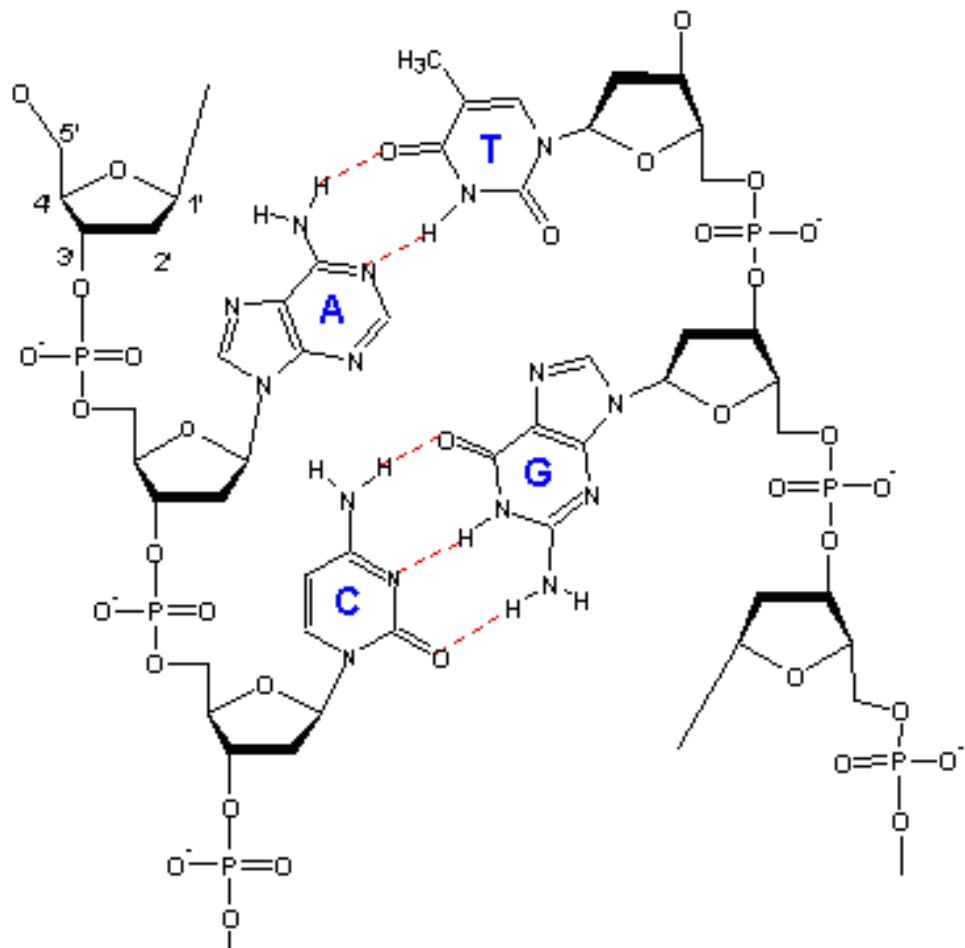
\includegraphics[width=0.63\textwidth]{adn.jpg}

\caption[Représentation de l'ADN]{Structure chimique de l'ADN. Le squelette est composé d'une succession de phosphates et de sucres liés entre eux. Chacun des sucres est de plus lié à une base azotée. Les bases azotées peuvent interagir par liaisons hydrogènes et interactions orbitalaires. Les bases s'associent plus facilement avec leur complémentaire (Adénine et Thymine ou Cytosine et Guanine) permettant une certaine variété de structure: repliement d'ADN simple brins ou encore association de deux cha\^{i}nes complémentaires formant l'hélice caractéristique de l'ADN dit double brins (image empruntée au cours de Sergei N. Smirnov \cite{adnjpg}).}
\label{adn}
\end{center}
\end{figure}

La structure chimique de l'ADN et ses interactions (rappelées sur la figure \ref{adn}) génèrent des propriétés qui sont fortement dépendantes de la séquence. L'influence de la séquence et la compréhension du vivant passe par la capacité à séquencer l'ADN, c'est à dire déterminer l'enchaînement des nucléotides. \\

Les applications sont potentiellement nombreuses: caractérisation d'espèces vivantes \cite{Sanggaard2014}, identification de souches pathogènes pour les virus ou bactéries \cite{Janda2007}, diagnostique des maladies génétiques \cite{Saunders2012}, étude de la phylogénie \cite{Neves2011}, analyse de la résistance aux antibiotiques  \cite{Davies2010}, identification de mutations \cite{Schneeberger2009}, médecine personnalisée \cite{Hamburg2010}, identification d'individu pour la police scientifique \cite{Wilson1995}.\\


Dès la deuxième moitié des années 70, les premières méthodes de séquençage voient le jours. Il s'agit de la méthode de Sanger \cite{Sanger1975} (voir figure \ref{sangermethod}) basée sur une synthèse enzymatique sélective (inspirée des travaux de Wu et al \cite{WU1972}, qui déterminèrent la première séquence de 24 paires de bases) et de la méthode Maxam et Gilbert \cite{Maxam1977} basée sur une dégradation chimique sélective. Gilbert et Sanger obtiennent tous les deux le prix Nobel de médecine en 1980 pour leurs méthodes. En 1977, grâce à sa méthode, Sanger parvient à séquencer le premier génome complet, il s'agit du bactériophage $\Phi$X174 \cite{Sanger1977}.\\

\begin{figure}[H]
\begin{center}
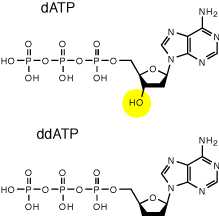
\includegraphics[width=0.5\textwidth]{ddatp.png}\hspace{1.3cm} 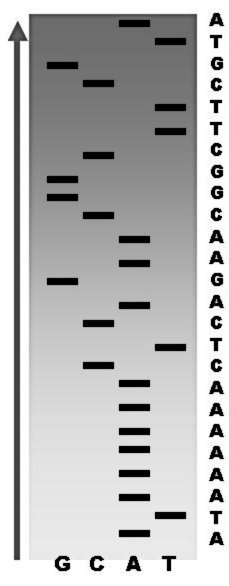
\includegraphics[width=0.21\textwidth]{gelelectrophoresis.jpg}
\vspace{0.5cm}

\caption[Séquencer par la méthode de Sanger]{Le séquençage par la méthode de Sanger : Le brin d'ADN à séquencer est répliqué parallèlement dans quatre milieux différents contenant chacun les quatre désoxyribonucléotides triphosphate (dATP, dCTP, dGTP, dTTP). Chacun des milieux présente en plus une faible quantité de l'un des didésoxynucléotides triphosphate (ddATP, ddCTP, ddGTP ou ddTTP), qui une fois incorporé dans la cha\^{i}ne empêche toute croissance supplémentaire (image de gauche). Chacun des quatre milieux présente alors des cha\^{i}nes de tailles variées terminant toutes par un même nucléotide. Les milieux sont alors analysés par électrophorèse sur gel, ce qui va trier les cha\^{i}nes par taille. On peut alors remonter à la séquence par lecture directe sur le gel (image de droite).}
\label{sangermethod}
\end{center}
\end{figure}



 
 La méthode de Sanger est rapidement préférée à celle de Maxam-Gilbert car elle nécessite moins de composés chimiques toxiques et de marqueurs radioactifs. Elle a été utilisée du début des années 80 jusqu'à la moitié des années 2000 avec principalement des avancées techniques:  marquage fluorescent \cite{Prober1987}, électrophorèse capillaire \cite{Swerdlow1991} ou encore automatisation des procédures \cite{Hunkapiller1991}.\\
 
  Afin de séquencer de longs génomes, les nouvelles techniques utilisent la méthode dite shotgun, élaborée par R. Staden \cite{Staden1979}, qui reconstruit un génome complet à partir de fragments de séquences moins coûteux et plus simples à séquencer (voir figure \ref{shotgun}).
 


\begin{figure}[H]
\begin{center}
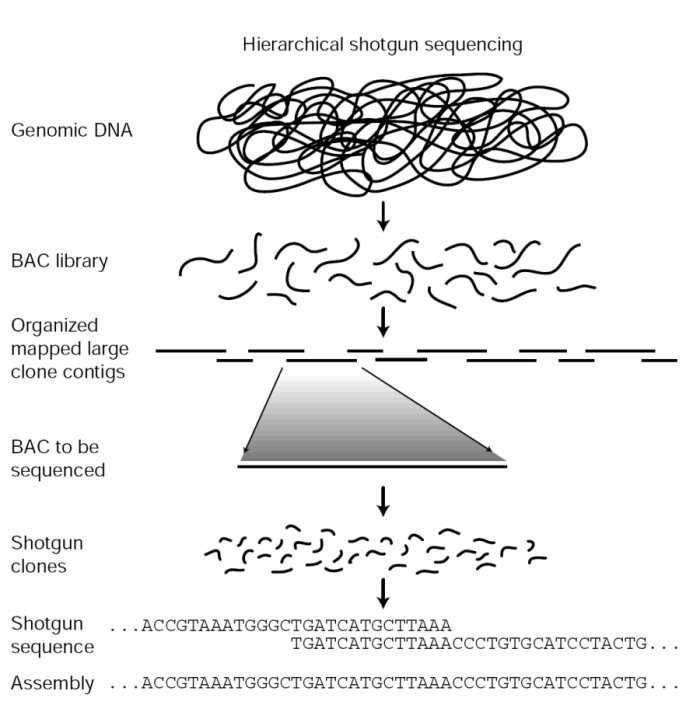
\includegraphics[width=0.75\textwidth]{shotgun.jpeg}
\vspace{0.5cm}

\caption[Méthode Shotgun]{Schéma de principe de la méthode shotgun (emprunt à l'article de revue de Eric S. Lander et al.\cite{Lander2001}). Le brin étudié est d'abord copié de nombreuses fois par PCR. Les brins sont ensuite fragmentés pour créer une banque de séquences aléatoires plus courtes (et moins compliquées à séquencer) qui sont également marquées. Ces fragments subissent à nouveau une PCR et forment de nombreux clones rassemblés chacun dans une colonie (ou polonie, contraction de PCR et colonie, voir figure \ref{pcr}). Chaque colonie est alors séquencée. De lourds traitements informatiques sont enfin employés pour reconstituer la séquence d'origine à partir des parties de génomes qui se chevauchent entre séquences.}
\label{shotgun}
\end{center}
\end{figure}

 En plus de nécessiter une librairie de base, ces techniques impliquent une amplification du signal ADN de départ par PCR (Polymerase Chain Reaction) \cite{Saiki1985}, de lourd traitements algorithmiques et sont sujettes à des erreurs notamment en ce qui concerne les parties de séquences redondantes dont certaines peuvent être omises. 


 \begin{figure}[H]
\begin{center}
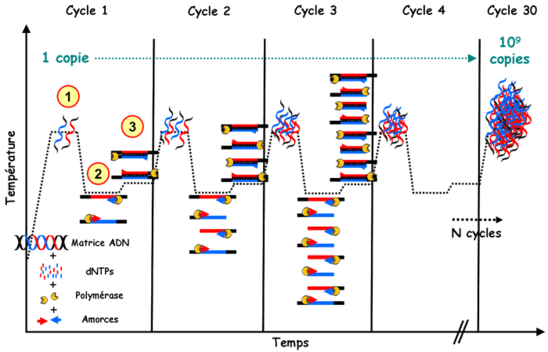
\includegraphics[width=0.85\textwidth]{pcr.png}

\vspace{0.5cm}

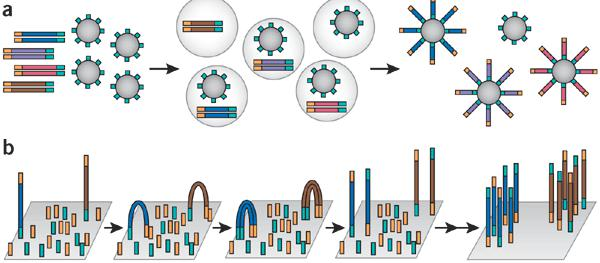
\includegraphics[width=0.85\textwidth]{bridgepcr.jpg}
\vspace{0.5cm}

\caption[PCR]{En haut, schéma de principe d'une PCR (Polymerase Chain Reaction), emprunt au site de l'université de Strasbourg \cite{pcrjpg}. Plusieurs cycles sont effectuées dans un milieu contenant la séquence à répliquer, des oligonucléotides amorces spécifiques, des polymérases et des nucléotides. La température est élevée jusqu'à 95°C pour dénaturé l'ADN et le rendre simple brin, elle est ensuite baissée entre 45 et 70°C pour que les amorces s'arriment aux brins de séquence à reproduire, et enfin la température est ré-élevée à 72°C pour réaliser la croissance des brins complémentaires par la polymérase. En bas, illustration de l'article de revue de Shendure \cite{Shendure2008}. a/ Une PCR réalisée en émulsion, les cycles successifs de température sont réalisés au sein d'une goûte en suspension. b/ Une PCR sur lame de microscope, la multiplication de l'ADN a lieu sur une zone restreinte grâce à un système de liaison covalentes avec les amorces de la réaction. Chaque goutte en suspension ou chaque zone sur la lame de microscope est appelée colonie d'ADN (ou polonie, contraction de PCR et colonie). Une polonie contient un unique fragment de la banque d'ADN. Les différents appareils commerciaux se distingueront dans un premier temps uniquement dans la façon d'effectuer la PCR et/ou de séquencer ces polonies.}
\label{pcr}
\end{center}
\end{figure}

Deux types de PCR seront successivement utilisées. La PCR en émulsion \cite{Williams2006}, puis la PCR directement sur lames de microscopes \cite{Shendure2005}. La figure \ref{pcr} présente le concept de PCR et ces deux exemples. Cette première génération de séquençage a permis en 2001 le premier séquençage complet du génome humain \cite{Lander2001,Venter2001}, Graal du Human Genome Project pour un coût total estimé de 3 milliards de dollars \cite{adncost}.


Brevetées dans les années 90 \cite{tsien1991dna,farinelli1998method}, les méthodes précédemment décrites vont être utilisées dans des appareils de séquençage commerciaux, ce qui va populariser l'utilisation du séquençage \cite{Schuster2007}. Ces appareils se distinguent principalement par les moyens utilisés afin de séquencer la banque d'ADN obtenue dans le cadre de la méthode shotgun. Le premier appareil de cette génération, le MPSS (Massively parallel signature sequencing \cite{Brenner2000}) voit le jour en 2000. Il repose sur une méthode tellement complexe qu'aucun appareil n'a été fourni à des laboratoires indépendants, les séquençages ayant lieux dans les locaux de la compagnie Lynx Therapeutics.

 D'autres appareils sont développés en parallèle. En 1996 le pyrosequencing \cite{Ronaghi1996}, séquençage qui repose sur la détection de l'activité de l'ADN polymérase par un pyrophosphate voit le jour. Ce procédé sera utilisé par un appareil commercial de la société 454 Life Sciences en 2005 \cite{Margulies2005}. Life Technologies avec le séquençage SOLiD \cite{mckernan2007reagents,Cloonan2008} (Sequencing by Oligonucleotide Ligation and Detection) commercialise son appareil en 2008. Il s'agit de séquençage par ligation, ce dernier repose sur une identification de la séquence par la forte spécificité de l'ADN ligase, qui va lier à l'aide d'une séquence de référence, un brin complémentaire, préalablement marqué, à la séquence inconnue. La partie liée est caractéristique de deux bases successives. 
% Quatre flurophores différents sont utilisés et chacun des fluorophores est donc caractéristique de quatre doublets de bases ( il y en a $2^{4}=16$ différents répartis sur quatre fluorophores).
 Des lectures successives en décalant les ligations d'une base permettent de déduire la séquence. Ce système a vu le jour dans un premier temps avec une PCR en émulsion puis une version utilisant une PCR sur support solide a été développée. Cette technique est efficace mais présente cependant des erreurs lors de la lecture de séquences formant des palindromes \cite{Huang2012}.
 
  La société Illumina en 2008 \cite{Bentley2008} sort le premier appareil basé sur une PCR sur support solide. Le séquençage est réalisé par la lecture de fluorophores lors de l’incorporation de bases modifiées au cours de la PCR. Le marquage est retiré à chaque étape de lecture. Life Technologies utilise quant à elle aussi le séquençage par semi conducteurs pour détecter les ions hydrogènes relâchés lors de la polymérisation de l'ADN (Ion semiconductor sequencing) \cite{Rusk2010}. Cette méthode est efficace, mais rencontre des  problèmes avec les répétitions d'homopolymères \cite{Rusk2010}. 

\begin{figure}[H]
\begin{center}
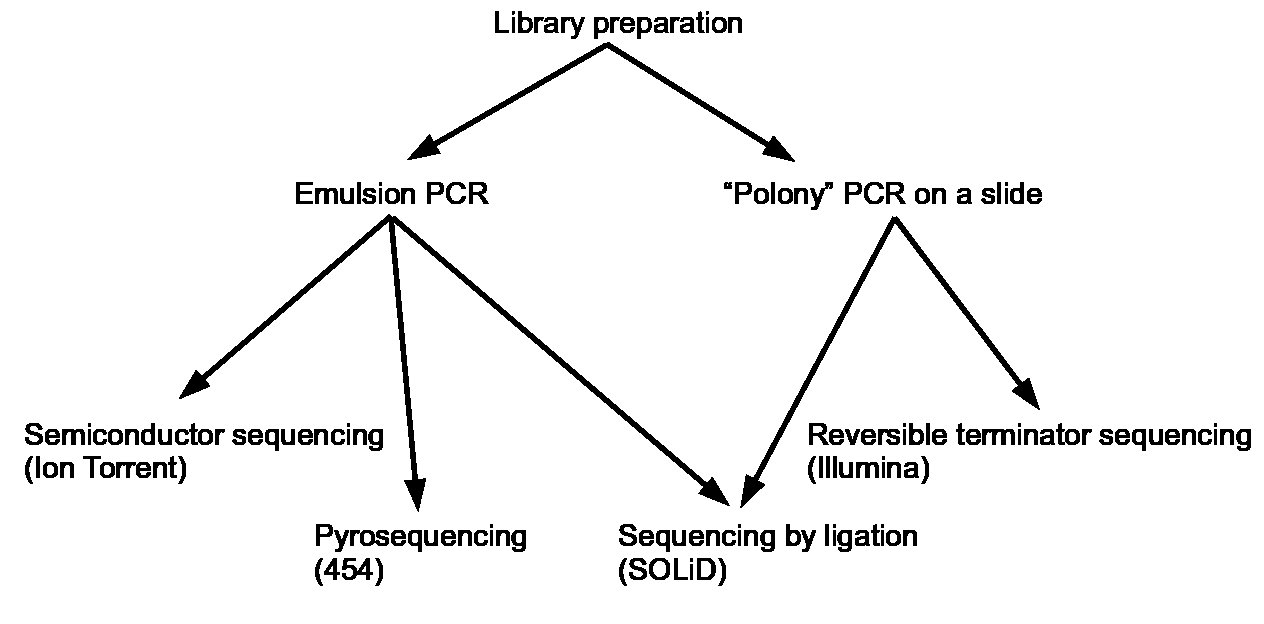
\includegraphics[width=0.8\textwidth]{ngsprinciple.jpg}
\vspace{0.5cm}

\caption[Principe du séquençage nouvelle génération]{Schéma récapitulatif du fonctionnement des premiers appareils de séquençage de nouvelle génération \cite{ngsprinciplejpg}.}
\label{ngsprinciple}
\end{center}
\end{figure}

Comme nous l'avons vu, ces procédés nécessitent une PCR pour amplifier le signal ADN de départ. Cette étape est source d'erreurs, en effet la PCR peut être biaisée et peut générer des artefacts \cite{Acinas2005}.



Deux autres techniques de lecture sans amplification sont développées, DNA nanoball sequencing \cite{Porreca2010} et Heliscope single molecule sequencing \cite{pmid20890904}, mais restent peu utilisées car elles ne sont utilisables que sur des fragments d'ADN très courts. Une approche originale est également commercialisée, il s'agit du séquençage en temps réel d'une molécule unique (Single molecule real time sequencing), un marquage fluorescent est détecté lors de la création du brin complémentaire lors de la copie de l'ADN \cite{Eid2009}. Cependant plusieurs lectures sont nécessaire pour obtenir une précision suffisante \cite{Chin2013}. Ces derniers appareils sont précurseurs de la troisième génération de séquençage en manipulant des molécules uniques.



Certains de ces appareils sont comparés dans les articles de revue de Quail et al. \cite{Quail2012} et de Liu et al. \cite{Liu2012}. 

\begin{figure}[H]
\begin{center}
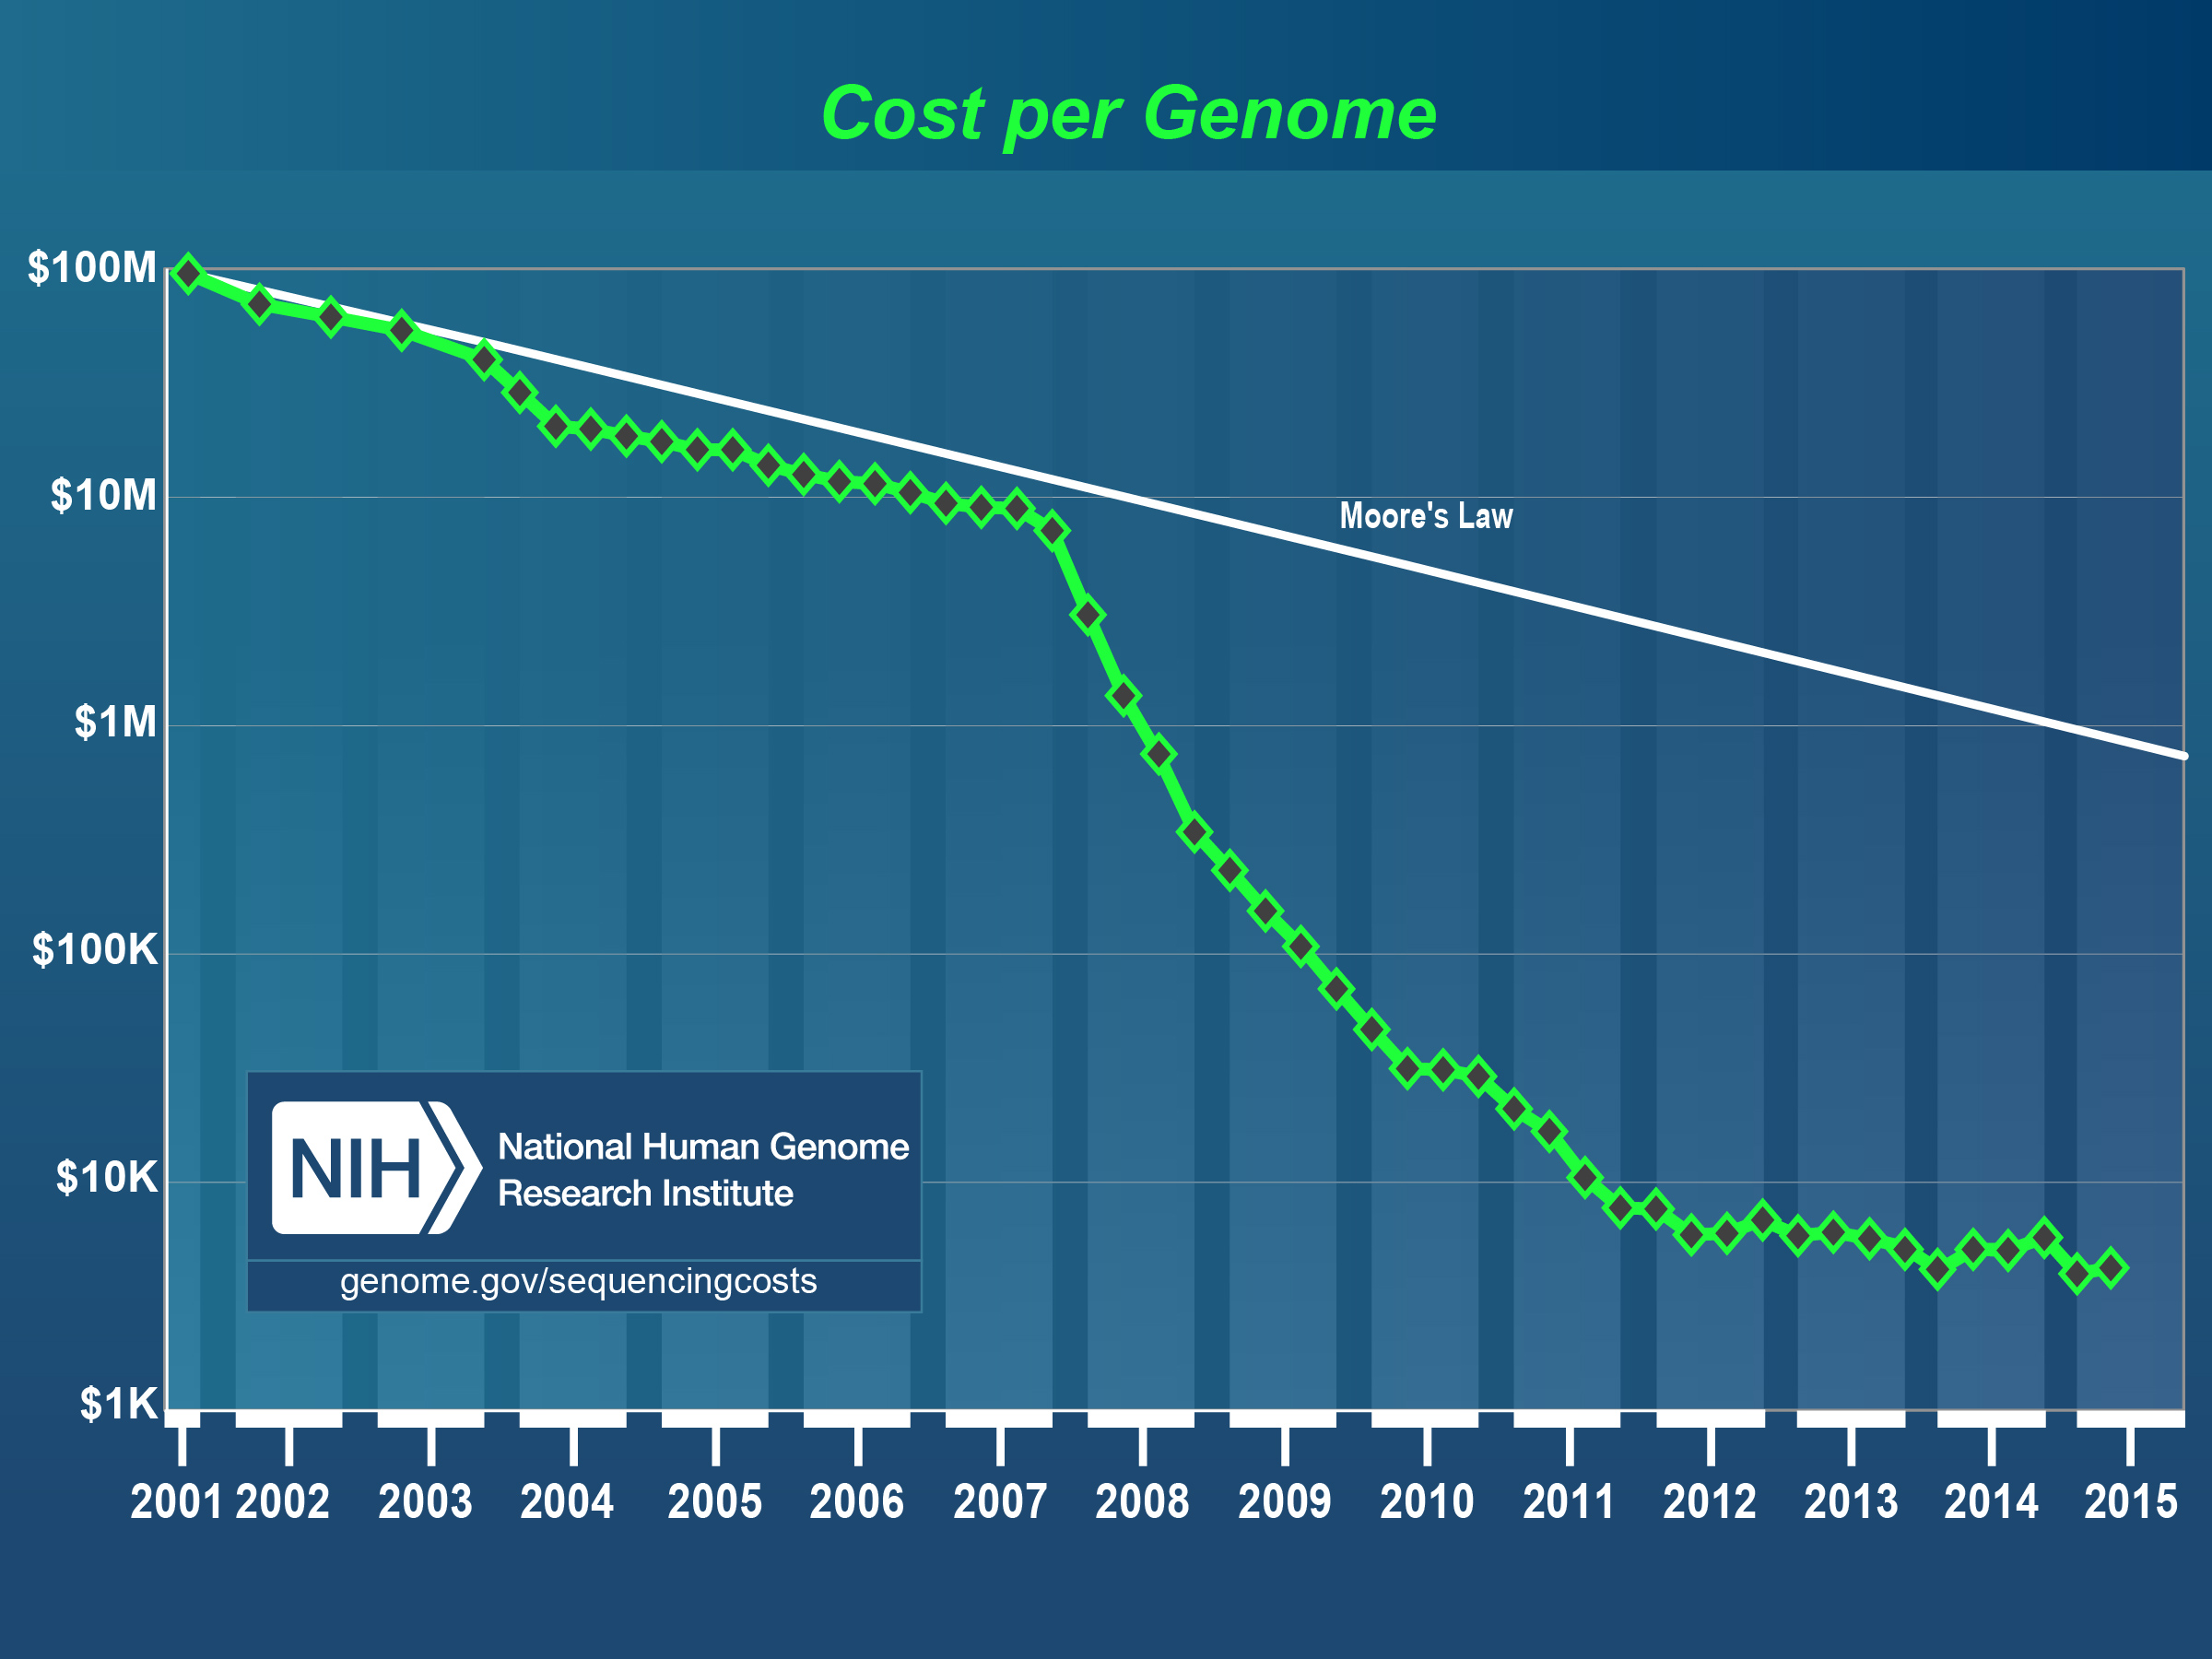
\includegraphics[width=0.7\textwidth]{cost_genome.jpg}

\caption[Coût du séquençage]{Evolution du coût du séquençage d'un génome complet selon le NIH \cite{adncost}. On observe au départ une diminution normale du coût suivant une loi de Moore. L'arrivée des premiers appareils commerciaux de séquençage de nouvelle génération se traduit par une rupture de pente très nette en 2007. Aujourd'hui, un plateau au dessus de l'objectif des 1000 USD pour un génome complet est atteint, d'où la nécessité de développer des méthodes dites de troisième génération.}
\label{seqcost}
\end{center}
\end{figure}


Tous ces appareils commerciaux  ont fait leurs preuves mais leur utilisation demeure trop coûteuse pour envisager leur usage à grande échelle. Une troisième génération de technique de séquençage est aujourd'hui envisagée. La figure \ref{seqcost} présente l'évolution du coût du séquençage d'un génome complet. Nous sommes toujours au dessus de l'objectif de 1000 USD \cite{Mardis2006}.
\\

Voici une liste de pistes envisagées pour les appareils de séquençage de troisième génération:

\begin{itemize}


\item Le séquençage par hybridation \cite{Zhang2003}. Ce procédé permet de reconnaître des séquences types par leur hybridation avec des bio-puces à ADN (de courtes séquences), cela nécessite un marquage fluorescent ainsi qu'un nombre important de produits chimiques et d'ADN de base.

\item L'utilisation de la spectroscopie de masse \cite{Edwards2005}. Basée sur la différence de masse entre les nucléotides, cette méthode semble être adaptée à la détection de substitution de bases dans différents gênes, mais pas pour séquencer des génomes de novo (dans leur intégralité). Elle s'avère utile cependant pour la médecine légale \cite{Howard2013}. 

\item La mise au point de techniques de microscopie électronique \cite{Bell2012}. Ces techniques sont complexes car elles nécessitent une modification des bases de l'ADN pour incorporer des atomes au numéro atomique élevé, afin d'obtenir un contraste suffisant.

\item La manipulation de bio-molécules avec pinces optiques, magnétiques ou AFM \cite{Pareek2011,Ding2012}.

\item La mesure du courant obtenu par effet tunnel lors du passage de l'ADN dans un canal microfluidique \cite{Ohshiro2012,DiVentra2013}.

\item \textbf{Le séquençage par nanopore.}


\end{itemize}


C'est cette dernière possibilité que nous explorons !

\subsection{Utilisation de nanopores et types de pores}

Le séquençage par nanopore a potentiellement de nombreux avantages sur les systèmes commerciaux déjà existants. En effet, cette technique laisse envisager la lecture de longues séquences (supérieurs à 5000 paires de bases) à vitesse élevée (1 paire de base par nanoseconde) \cite{Timp2010,Branton2008}. Aucun marquage chimique n'est nécessaire, l'utilisation d'enzymes est moindre et le signal ADN n'a pas besoin d'être amplifié (pas de PCR).

Exposons dans un premier temps les concepts de bases et définitions du séquençage par nanopore. On envisage de séquencer la séquence ADN au cours de sa translocation. Il s'agit du passage d'un polymère d'un coté, appelé cis, d'une membrane à l'autre, appelé trans, à travers un pore (voir figure \ref{translocbase}). Cette translocation peut être naturelle (non biaisée) ou pilotée par une force (biaisée). La translocation est un phénomène biologique fréquent, c'est le cas par exemple lorsqu'un virus infecte une cellule en y translocant son ADN.

\begin{figure}[H]
\begin{center}
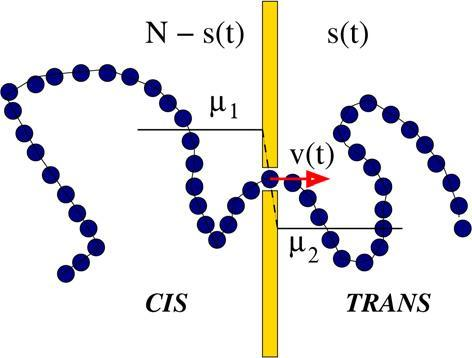
\includegraphics[width=0.44\textwidth]{translocation.jpg} 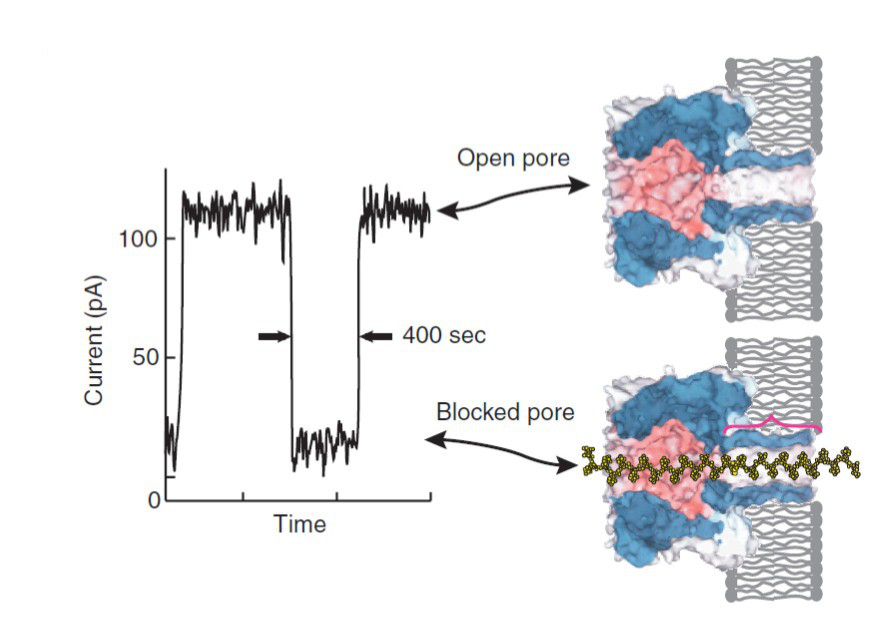
\includegraphics[width=0.55\textwidth]{translocissues.jpg}

\caption[Translocation et courant de blocage]{Translocation d'un polymère. A gauche: Illustration de la translocation biaisée d'un polymère par l'application d'une différence de potentiel chimique empruntée à l'article de revue de A. Milchev \cite{Milchev2011}. A droite: Translocation d'ADN à travers un bio-pore et mesure du courant de translocation illustrés par Branton et al. \cite{Branton2008}.}
\label{translocbase}
\end{center}
\end{figure}

Au cours de la translocation de l'ADN, on espère pouvoir séquencer en mesurant le courant de translocation. Le principe est simple, au cours de la translocation, l'occupation du pore entraîne une modification de sa résistance électrique, modification caractéristique de l'entité occupant ce pore. On peut alors espérer déterminer la nature de l'occupant du pore (typiquement la séquence pour l'ADN) en mesurant le courant ionique de blocage du pore (voir figure \ref{translocbase}). On dispose déjà de certaines applications de ce procédé, notamment pour le comptage de polymères \cite{Bezrukov1994}, la détection d'ADN et ARN \cite{Kasianowicz1996} ou encore la discrimination de certains polynucléotides \cite{Akeson1999,Meller2000,Ashkenasy2005}. Cette technique bien que prometteuse admet des limites de résolution spatiales et temporelles qui font qu'elle ne permettra pas de séquencer l'ADN \cite{Branton2008}. Nous expliquerons ces limites en décrivant les différent types de nanopores disponibles ainsi que les techniques alternatives qui s'inspirent de la mesure du courant ionique de blocage, dans le paragraphe suivant.

%\textcolor{red}{c'est démontré que courant ionique classique ne peut pas distinguer donc courant transverse ou fonctionnalisation. j en parlerais après description des différents nanopores.}

\subsubsection{Les biopores}


Historiquement, les premier nanopores utilisés sont ceux fournis par la nature. On peut employer la protéine F située sur la membrane extérieure de Escherichia Coli \cite{Danelon2006,Chimerel2008}) ou encore l'$\alpha$-hémolysine du Staphylocoque doré \cite{Bhakdi01121991}. Ce dernier est très utilisé car il est disponible commercialement, d'une reproductibilité parfaite et susceptible d'être employé avec de l'ingénierie génétique pour modifier certaines propriétés (blocage au passage d'ADN par exemple \cite{Howorka2001}). Il s'agit d'ailleurs du bio-pore utilisé par Kasianowicz et al. pour effectuer en 1995 la première translocation d'ADN \cite{Kasianowicz1996}.


\begin{figure}[H]
\begin{center}
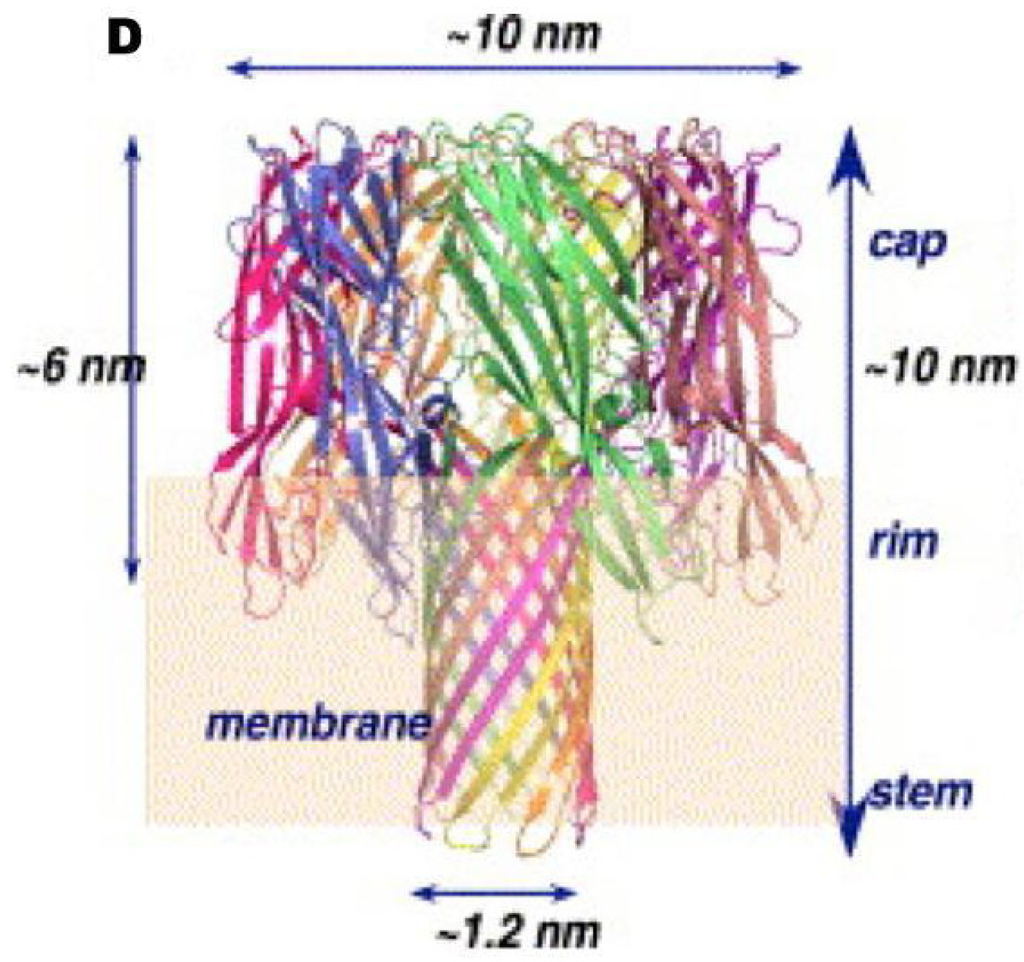
\includegraphics[width=0.51\textwidth]{bioporetoxine.png}
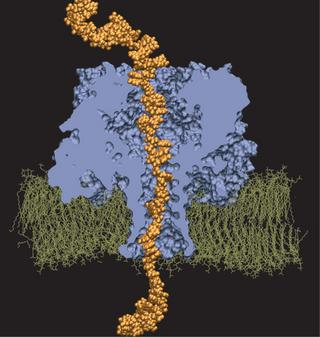
\includegraphics[width=0.42\textwidth]{biopore2.jpg}

\caption[Biopores]{Les bio-pores ont été les premiers pores utilisés à des fins d'étude ou d'emploi des phénomènes de translocation. A gauche, modèle du pore heptameric de B. cereus \cite{Ramarao2013}. A droite, simulation de translocation d'ADN à travers un bio-pore ($\alpha$-hémolysine) \cite{Aksimentiev2010}.}
\label{biopore}
\end{center}
\end{figure}


Ces bio-pores ont prouvé leur efficacité pour la translocation d'ADN et ARN simples brins ou encore pour des protéines dépliées \cite{Movileanu2005}. Ils demeurent trop étroit pour les formats double brins car leur diamètre n'est pas réglable. La nature fournie des outils efficaces, car avec l'utilisation en complément de protéines chaperonnes, il est possible d’empêcher l'inversion de la translocation \cite{DeLosRios2006} (phénomène qui inspira la fonctionalisation des autres types de pores dont nous allons parler par la suite). La figure \ref{bioporepossib} présente un inventaire succins des possibilitées offertes par les bio-pores. 
\begin{figure}[H]
\begin{center}
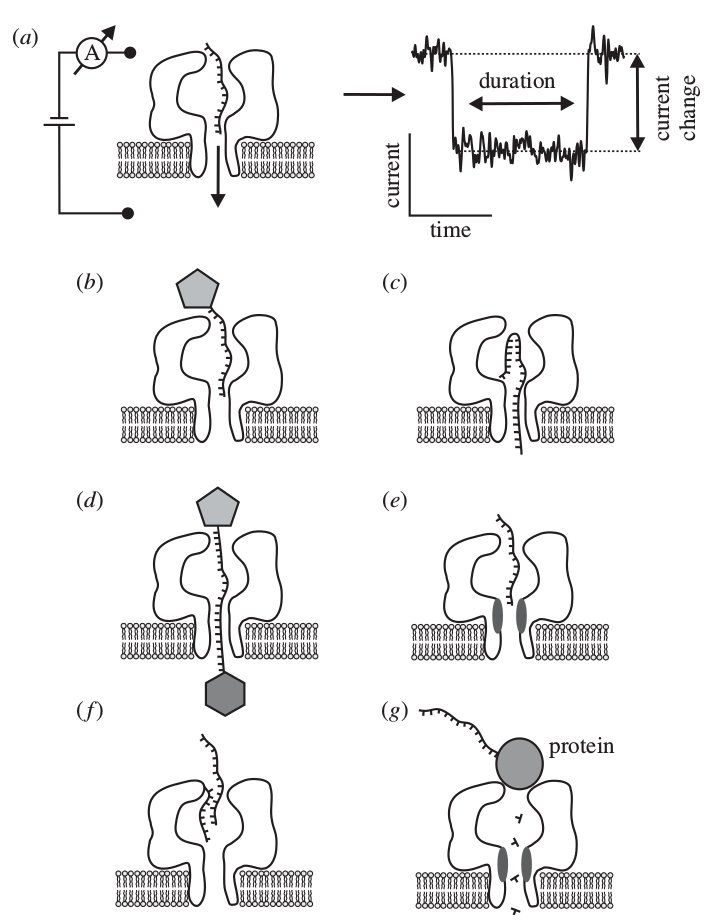
\includegraphics[width=0.85\textwidth]{bionanopore.jpg}


\caption[Manipulations sur bio-pores]{Différentes manipulation possibles avec les bio-pores (emprunt à l'article de revue de U. F. Keyser \cite{keyser}). a/ Mesure du courant ionique de translocation. b/ Une protéine plus large que le pore fixée sur l'ADN permet d'imposer le sens de la translocation. c/ Un brin replié sur lui même peut stopper la translocation. d/ Attacher une protéine à chaque extrémité de l'ADN peut conduire à une translocation à durée infinie. e/ La modification génétique du pore peut affecter la translocation. f/ Le pore peut être fonctionnalisé avec de l'ADN complémentaire d'une séquence à détecter. g/ Une endonucléase peut être combinée au nanopore pour réaliser une translocation base par base.}
\label{bioporepossib}
\end{center}
\end{figure}

Pour effectuer une translocation forcée à travers des bio-pores, l'outil principal demeure l'électrophorèse (potentiel électrique) \cite{Kasianowicz1996,Henrickson2000}. 
Dans une optique de séquençage, ils sont trop épais pour permettre de discriminer les séquences en cours de translocation car au sein du pore, se situent simultanément plusieurs dizaines de bases.

 L'utilisation d'une endonucléase (suggérée sur la figure \ref{bioporepossib}) par la société Oxford Nanopore Technologies est une possibilité pour surmonter ce problème. Un appareil commercial a vu le jour au cours de la thèse \cite{Mikheyev2014} et commence à être testé et utilisé \cite{Goodwin2015,Jain2015,Urban2015}. Leur technologie est décliné en plusieurs appareils allant du système portable au système de gros débit en format plus imposant \cite{oxfordnanopore} (voir figure \ref{oxfordnanopore}). 


\begin{figure}[h!]
\begin{center}

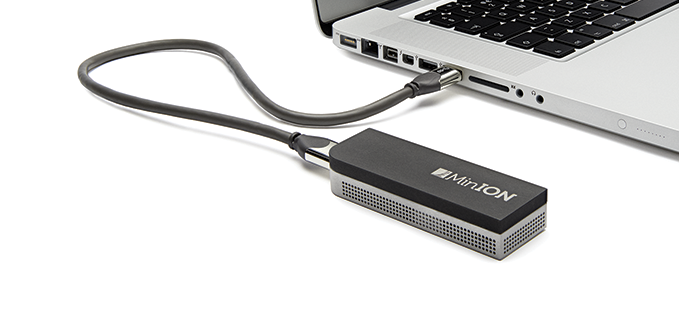
\includegraphics[width=0.5\textwidth]{MinION-Nanopore-technologies.png}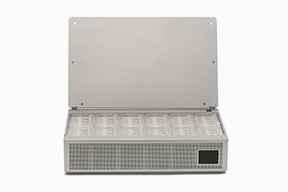
\includegraphics[width=0.5\textwidth]{PromethION-setup.jpg}

\caption[Séquenceur MinION]{Les appareils de séquençage, MinION et PromethION
de la société Oxford Nanopore Technologies \cite{oxfordnanopore}.}
\label{oxfordnanopore}

\end{center}
\end{figure}

Ces systèmes prometteurs présentent toujours des erreurs de lectures. Ces erreurs sont problématiques car la méthode est destructive pour l'échantillon. Afin de les contrôler il faudrait envisager une amplification du signal ADN de départ et donc l’utilisation de PCR et les mêmes inconvénients que nous avons vu précédemment. L'utilisation de bio-pores à des fins de séquençage est possible mais présente des contraintes auxquelles la communauté scientifique a rechercher un palliatif en développant des nanopores artificiels.



\subsubsection{Les premiers pores artificiels}


Les limites des bio-pores ont poussé les chercheurs à développer leur propres pores. En 2001 le premier nanopore artificiel est créé \cite{Li2001}. Un faisceau concentré d'ions ou d'électrons peut être utilisé pour creuser un pore dans une membrane de matériaux variés \cite{Wanunu2010}. Le silicium a été très utilisé. La figure \ref{artpore} illustre un pore typique vu par AFM.




\begin{figure}[h!]
\begin{center}
\begin{minipage}{0.45\linewidth}
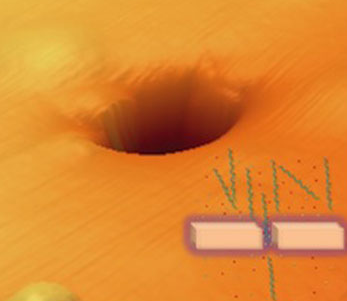
\includegraphics[width=\textwidth]{artificialpore.png}
\end{minipage}
\begin{minipage}{0.48\linewidth} 
\caption[Pores artificiels]{Vue par AFM d'un pore artificiel en silicium. Projet de l'université du texas \cite{artpore}. Bien que toujours épais, les nanopores de silicium présentent l'avantage d'être rigides, stables et de diamètres ajustables.}
\label{artpore}
\end{minipage}
\end{center}
\end{figure}

L'arrivée des nanopores artificiels a permis de travailler dans des conditions contrôlées. La possibilité de choisir le diamètre et les propriétés du pore s'accompagne du développement de techniques de manipulation pour forcer la translocation (voir la Figure \ref{solidstateporepossib}). L'électrophorèse est toujours possible \cite{Storm2005,2Storm2005,Wanunu2008}, cependant l'introduction des pores artificiels à également permis l'essort de l'utilisation de pinces magnétiques \cite{Peng2009} ou optiques \cite{Sischka2010}. Le ralentissement de la translocation en diminuant le diamètre du pore est également une possibilité \cite{Mirsaidov2010}. Afin de retrouver certaines propriétés des bio-pores, les pores artificiels peuvent aussi être fonctionalisés \cite{Mussi2010}. Certains ont même réalisé un couplage entre bio-pores et pore artificiels, en greffant une $\alpha$-hémolysine dans un nanopore de silicium \cite{Hall2010}, créant ainsi un pore hybride. La figure \ref{solidstateporepossib} montre les possibilités offertes par ces nanopore artificiels de première génération.


\begin{figure}[h!]
\begin{center}
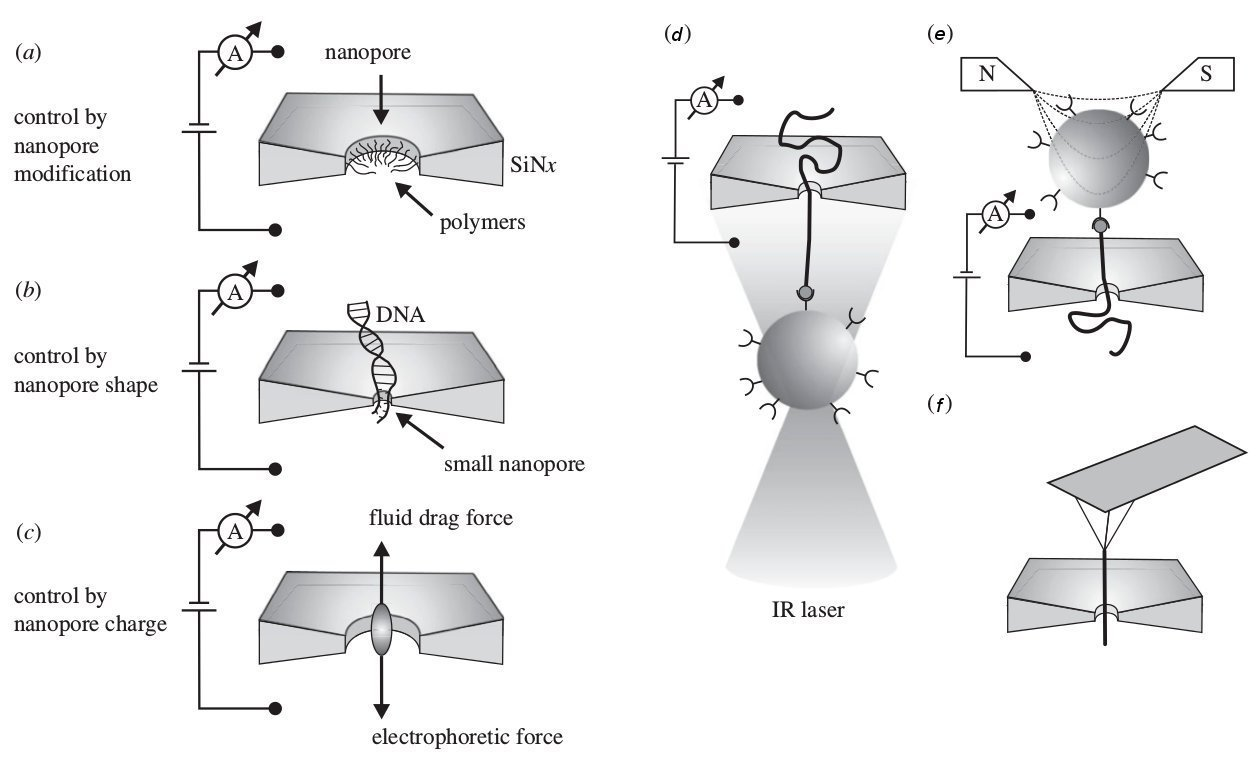
\includegraphics[width=1.0\textwidth]{solidstatenanopore.jpg}


\caption[Pores artificiels et manipulations]{A gauche, différentes modifications possibles avec les pores artificiels, à droite, les différents contrôles mécaniques possibles pour la translocation (emprunt à l'article de revue de U. F. Keyser \cite{keyser}). a/ Fonctionalisation du nanopore. b/ Gestion de la taille du nanopore. c/ Contrôle de la charge du pore (pouvant ralentir la translocation en générant une résistance hydrodynamique plus importante). d/ Utilisation de pinces optiques. e/ Utilisation de pinces magnétiques. f/ ADN accroché à une pointe d'AFM.}
\label{solidstateporepossib}
\end{center}
\end{figure}



Cette première génération de nanopores artificiels a permis d'effectuer des études quantitatives en variant certain paramètres, mais elle ne permet pas de relever le défi du séquençage non destructif. En effet l'épaisseur de ces dernier reste trop importante pour permettre la discrimination des séquences au cours de la translocation. Ceci fût un frein, jusqu'à l'isolation du graphène en 2004 par Andre Geim et Konstantin Novoselov \cite{Novoselov2004}. Ces derniers reçurent le prix Nobel de physique en 2010 pour leurs travaux sur le graphène.

\newpage

\subsubsection{Les pores artificiels fins}

L'arrivée du graphène marque le début d'une ère des possibles dans le domaine du séquençage par nanopores. En effet, le graphène étant un cristal bidimensionnel d'épaisseur mono-atomique stable, les problèmes de discrimination de la séquence au sein du pore sont potentiellement résolue par l'utilisation de membranes ultra fines. En 2010, Schneider et al. présentent la preuve expérimentale de la possibilité d'effectuer une translocation d'ADN à travers un nanopore dans une membrane de graphène\cite{Schneider2010}. L'utilisation du graphène présente de nouveau défis expérimentaux et théoriques car il présente, comme l'illustre la figure \ref{membvibgra}, des propriété vibrationnelles et est déformable.

\begin{figure}[h!]
\begin{center}
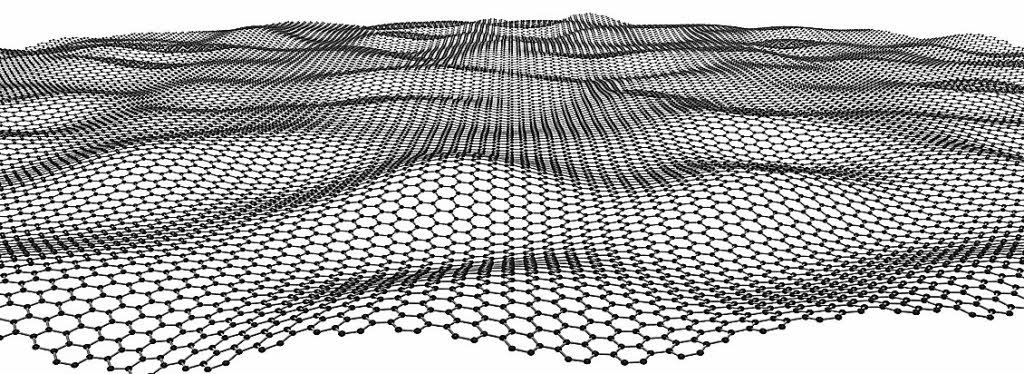
\includegraphics[width=0.84\textwidth]{vib.jpg}


\caption[Vibration et déformation d'une mono-couche de graphène]{Illustration de Jannik C. Meyer, qui a travaillé sur les membranes de graphènes \cite{Meyer2007}. La faible épaisseur des membranes monoatomiques entraîne une forte influence des vibrations, déformations et de la flexibilité.}
\label{membvibgra}
\end{center}
\end{figure}


Un autre cristal bidimensionnel est également envisagé, il s'agit du disulfure de molybdène \cite{Kang2014}, dans lequel des nanopores peuvent être creusés \cite{Feng2015} et une translocation effectuée \cite{2Feng2015}.

\begin{figure}[h!]
\begin{center}
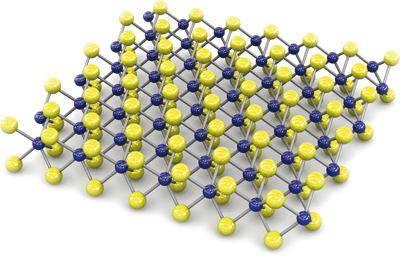
\includegraphics[width=0.78\textwidth]{MoS2.jpg}


\caption[Disulfure de molybdène]{Illustration de la structure du disulfure de molybdène \cite{Benameur2011}. Plus épais que le graphène, ce cristal bidimensionnel peut également être utilisé pour la translocation de polymères.}
\label{membvibmos2}
\end{center}
\end{figure}

Pour ces deux systèmes, il est possible d'effectuer une translocation mais sans pour autant pouvoir déterminer la séquence avec suffisamment de précision \cite{Schneider2010,2Feng2015}. Il est même possible d'envisager de créer des structures hybrides entre ces deux cristaux \cite{Roy2013}. Ces systèmes ont donc été modélisés pour voir comment améliorer la discrimonation des séquences (voir exemples de modèles sur la figure \ref{simultranslocboth}).

\begin{figure}[h!]
\begin{center}
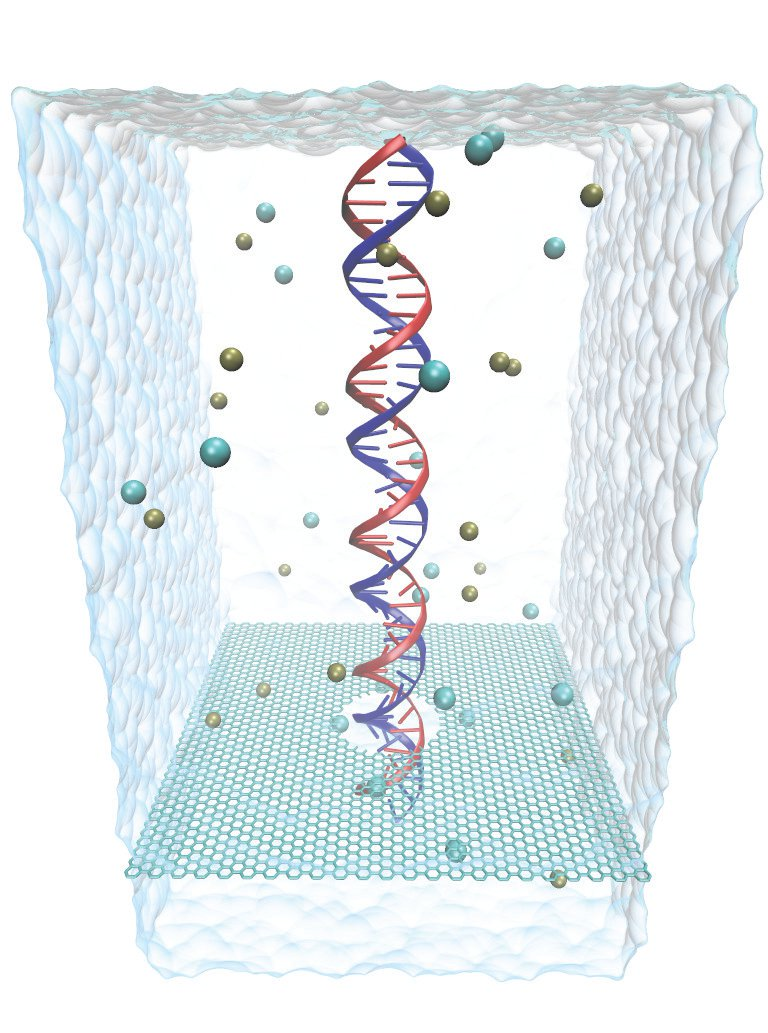
\includegraphics[width=0.45\textwidth]{dnatranslocsim.jpg}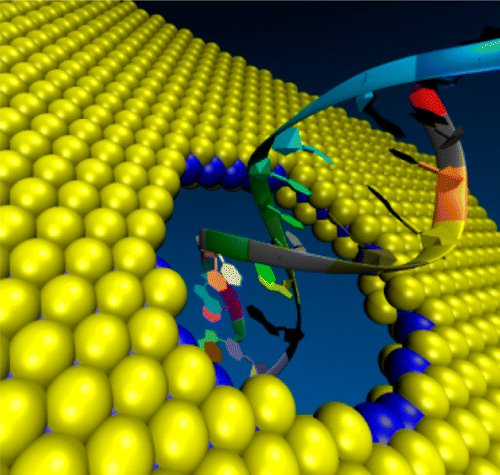
\includegraphics[width=0.55\textwidth]{mos2simul.jpg}

\caption[Translocation et cristaux bidimensionnels]{Simulations de la translocation d'ADN double brin à travers un nanopore dans des membranes de graphène \cite{Sathe2011} et de disulfure de molybdène \cite{Farimani2014}.}
\label{simultranslocboth}
\end{center}
\end{figure}

\newpage

\subsubsection{Les bio-pores fins}

En se basant sur la théorie développée par Seeman \cite{Seeman1982}, Rothemund a montré qu'il était possible de créer des Structures 2D d'ADN par autoassemblage \cite{Rothemund2006}. Le nom d'origami d'ADN a été donné à ses structures (pouvant également être développée à 3 dimensions \cite{Kuzuya2009}). Des exemples de structures 2D et 3D d'origami ADN sont présentés sur la figure \ref{origami}. 

\begin{figure}[H]
\begin{center}
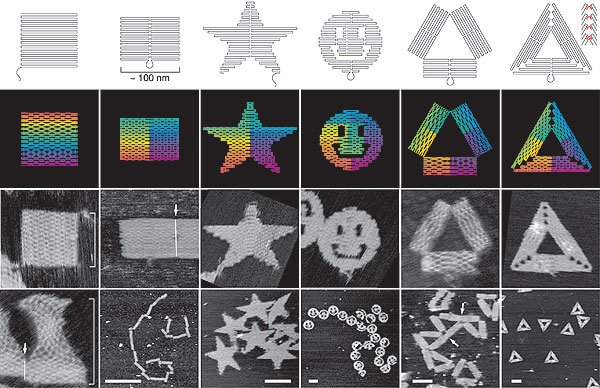
\includegraphics[width=0.8\textwidth]{origami2d.jpg}
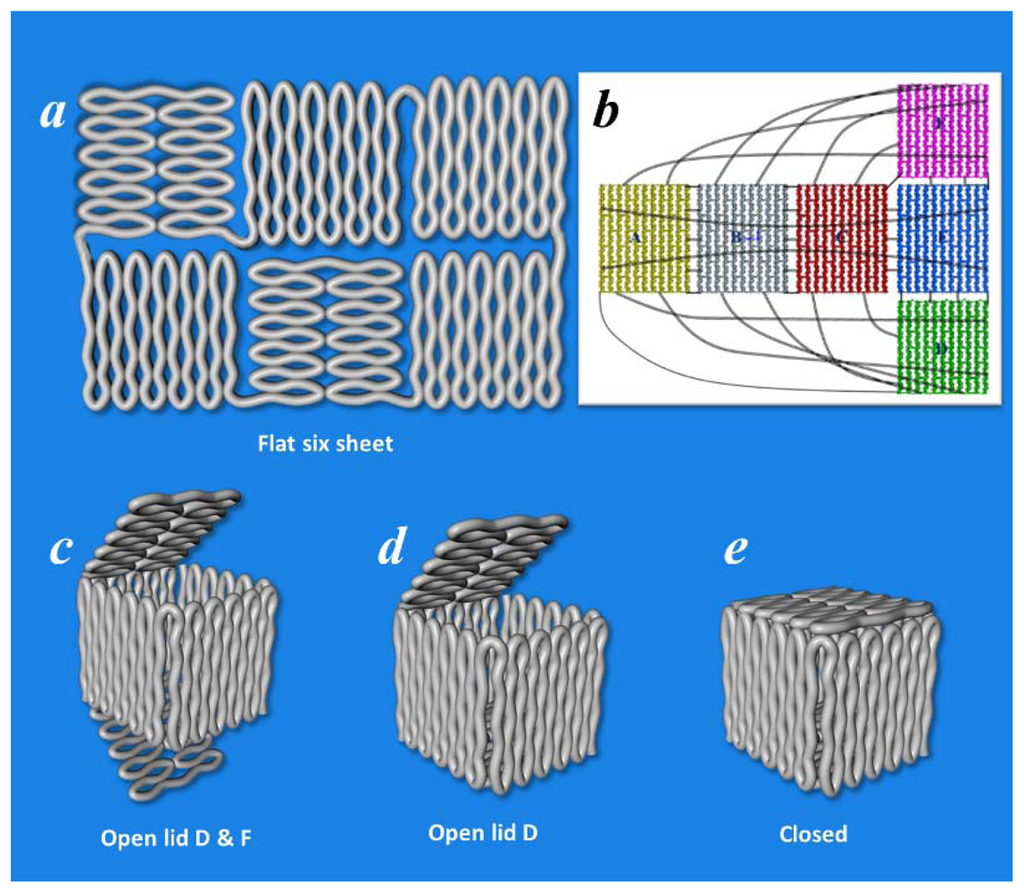
\includegraphics[width=0.8\textwidth]{origamis3d.png}

\caption[Origamis d'ADN]{Exemples de structures d'origamis ADN à 2\cite{Rothemund2006} et 3 dimensions \cite{Zadegan2012}.}
\label{origami}
\end{center}
\end{figure}

Ces structures d'ADN peuvent être utilisées afin de réaliser une membrane muni d'un nanopore \cite{2Bell2012}, au travers duquel il est possible d'effectuer la translocation d'un ADN \cite{HernndezAinsa2013}. de plus, comme l'illustre la figure \ref{origamitransloc}, ces pores peuvent être adaptés en taille et aisément fonctionnalisés.



\begin{figure}[H]
\begin{center}
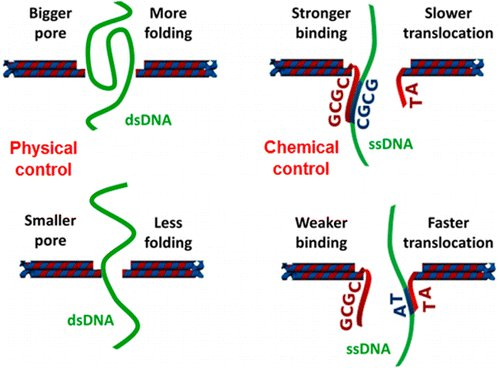
\includegraphics[width=0.8\textwidth]{origamitransloc.jpg}

\caption[Nanopore et origami d'ADN]{Un nanopore dans une membrane d'origami d'ADN \cite{HernndezAinsa2013}. Ce type de nanopore est de taille aisément adaptable et peut être fonctionnalisé facilement.}
\label{origamitransloc}
\end{center}
\end{figure}



Le fait de pouvoir travailler avec des membranes fines est une nouveauté qui laisse entrevoir une alternative à la mesure de courant ionique afin de déterminer la séquence de l'ADN en cours de translocation.





\newpage
\subsection{Mesures de courant et séquençage}

Comme nous l'avons vu précédemment, la mesure du courant ionique au cours de la translocation est l'idée maîtresse qui a guidé l'utilisation de nanopores afin de séquencer. Cependant l'arrivée des membranes fines laisse envisager une alternative: la mesure du courant transverse lors de la translocation. Illustrée sur la figure \ref{couranttransv1}


\begin{figure}[H]
\begin{center}
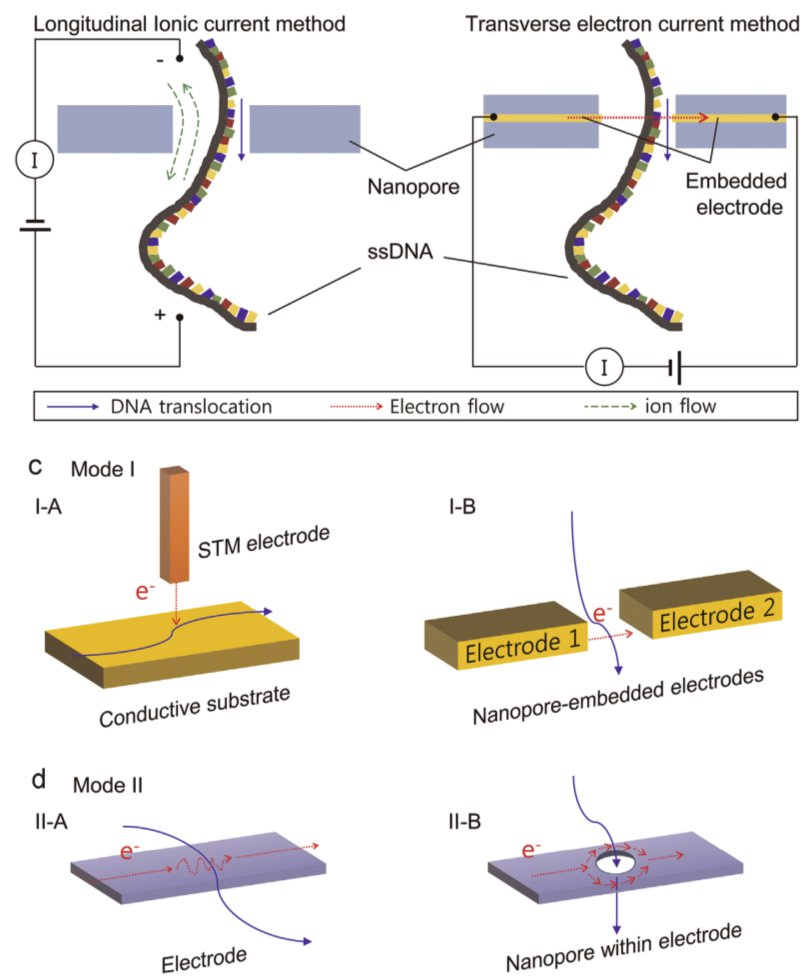
\includegraphics[width=0.8\textwidth]{introcouranttransverse.jpg}

\caption[Courants ioniques et transverses]{En plus de la mesure longitudiale du courant ionique lors de la translocation (a), il est possible avec les membranes fines de mesurer un courant électronique transverse (b) selon deux modes. Pour le premier mode (c), la translocation à lieu entre deux électrodes, alors que pour le deuxième mode (d), le nanopore est situé au sein d'une électrode.}
\label{couranttransv1}
\end{center}
\end{figure}

L'article de revue de Kim et al.\cite{Kim2015} présente plusieurs exemples de montages expérimentaux permettant de mesurer ce courant transverse (voir figure \ref{couranttransv2}). Les exemples donnés concernent le graphène mais il possible d'imaginer le même type de structure avec du sulfure de molybdène ou des origamis d'ADN dopés pour la conductivité.



\begin{figure}[H]
\begin{center}
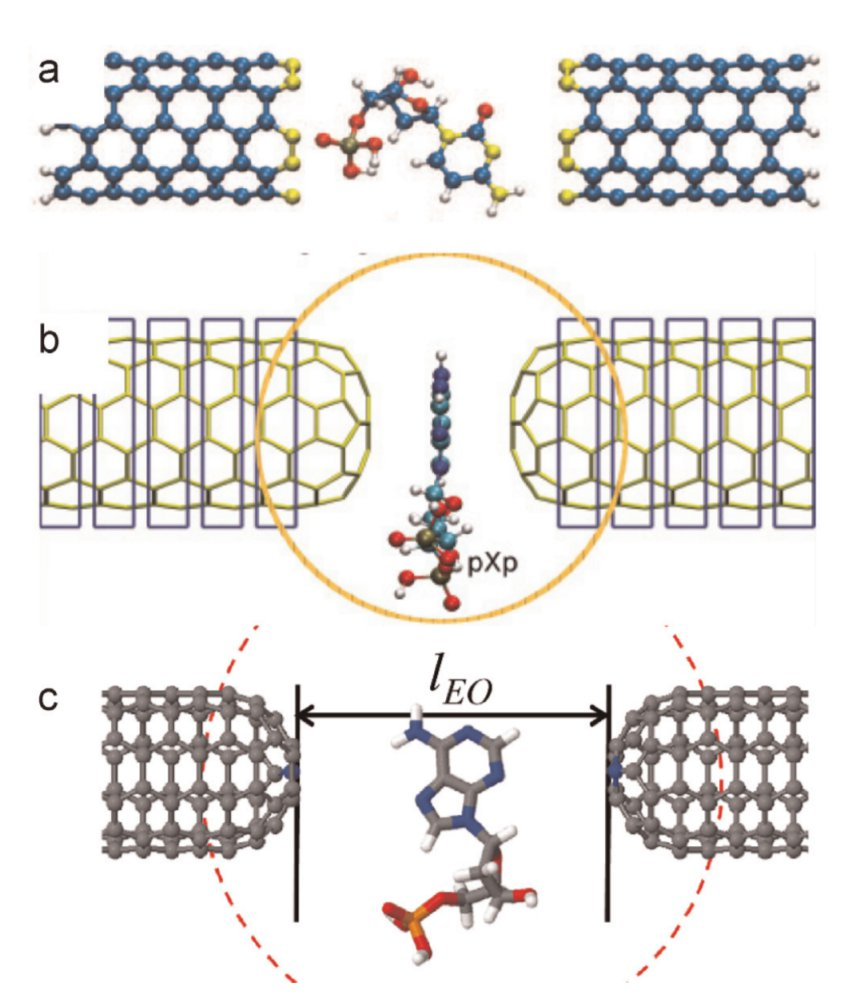
\includegraphics[width=0.7\textwidth]{couranttransv2.jpg}
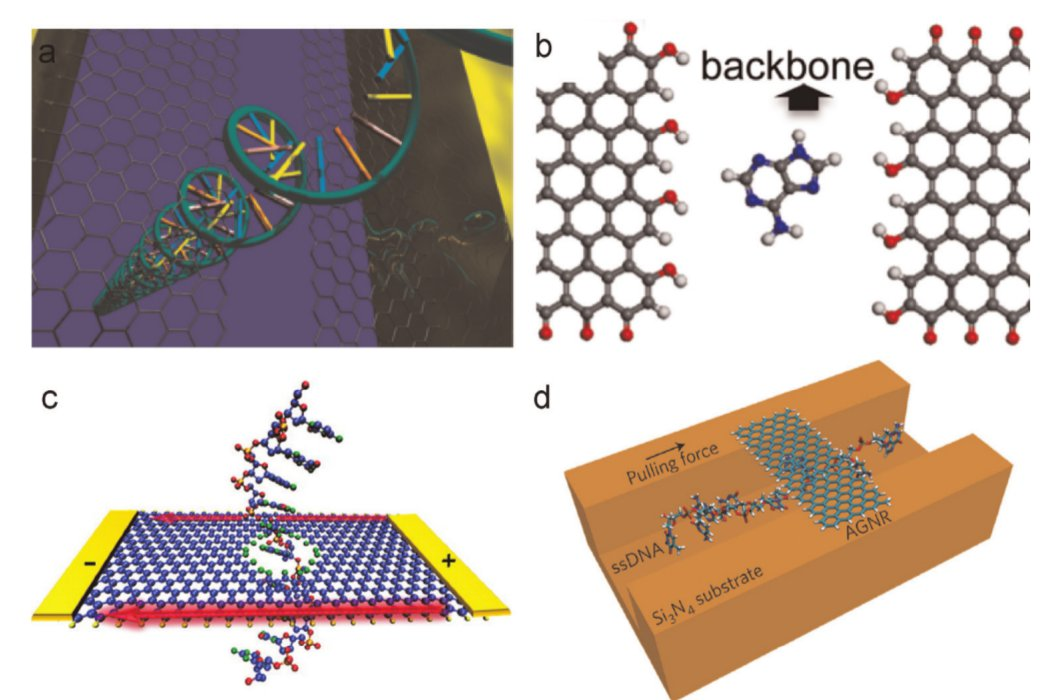
\includegraphics[width=0.7\textwidth]{couranttransv1.jpg}

\caption[Montages pour mesure du courant transverse]{Exemples de mesures de courant électroniques transverses lors de la translocation. En haut:  a/ membrane de graphène fonctionnalisée avec de l'azote \cite{Meunier2008} b/ nanotube de carbone utilisé comme membrane \cite{Chen2012} c/ nanotube de carbone fonctionnalisé avec de l'azote \cite{Kim2013}. En bas:  a/ nanopore constitué d'une bande \cite{Postma2010} b/ fonctionnalisation avec de l'oxygène \cite{Jeong2013} c/ nanopore au sein d'une électrode \cite{Saha2012} d/ Mesure de courant transverse perturbé par interactions orbitalaires \cite{Min2011}. Tous ces exemples concernent le premier mode sauf la figure c du bas qui montre un exemple de second mode.}
\label{couranttransv2}
\end{center}
\end{figure}







\section{Modélisation}


Après avoir vu le contexte technologique dans lequel s'inscrit le séquençage par nanopore, intéressons nous aux différentes manières de modéliser ce problème.





\subsection{Modèles théoriques}

Comme nous venons de le voir, l'utilisation de la translocation de l'ADN à des fins de séquençage est prometteur. Ce potentiel a créer un certain engouement au sein de la communauté scientifique. Dès 1996  Sung et Park proposent une première approche théorique de la translocation \cite{Sung1996} poursuivie en 1999 par Muthukumar \cite{Muthukumar1999}. Ils calculent une barrière d'énergie à franchir au cours de la translocation et proposent de résoudre l'équation de Fokker-Planck (propre des systèmes diffusifs \cite{shiriaev1992selected}). L'ADN, comme tout polymère, suit des lois générales de physique statistique (voir les travaux du prix Nobel Pierre-Gilles de Gennes \cite{Gennes197911} et notre \hyperref[resideal]{deuxième chapitre} qui y consacre une bonne partie), la difficulté réside dans le fait que pour la translocation, les conditions d'équilibres sont rarement remplies et de nombreuses tentatives d'explications théoriques ont eu lieu. Le \hyperref[translocmurfixe]{chapitre 3} consacre un long chapitre à toutes les théories développées afin de comprendre la translocation des polymères. Une approche théorique peut également être entreprise afin de prédire les courant ioniques au cours de la translocation \cite{Im2002,Noskov2004,Saraniti2006}. La comparaison aux expériences n'est pas toujours évidente et la mise en place de modèles numérique est nécessaire pour comprendre toutes les subtilités du problème.




\subsection{Echelles des modèles numériques}


Puisque l'ADN est un polymère  et en tant que tel suit des lois communes à tous les polymères, mais il présente également des propriétés qui lui sont propres. Pour attaquer le problème de la translocation, il faut d'abord choisir le niveau de détail souhaité. Si l'on souhaite comprendre le problème de la translocation de polymères en générale, des modèles simples, avec un faible niveau de détails, suffisent. Si l'on s'intéresse à la translocation d'une séquence particulière dans un pore ayant ses particularités, un niveau de détail fin, typiquement un modèle tout atomes, est nécessaire. De même si l'on souhaite déterminer le courant de translocation attendu. On peut également se situer à des échelles intermédiaires qui peuvent être un bon compromis, c'est le cas des modèles dit gros grains. La figure \ref{echellemodeles} présente trois modèles de niveaux de détails croissants.

\begin{figure}[H]
\begin{center}
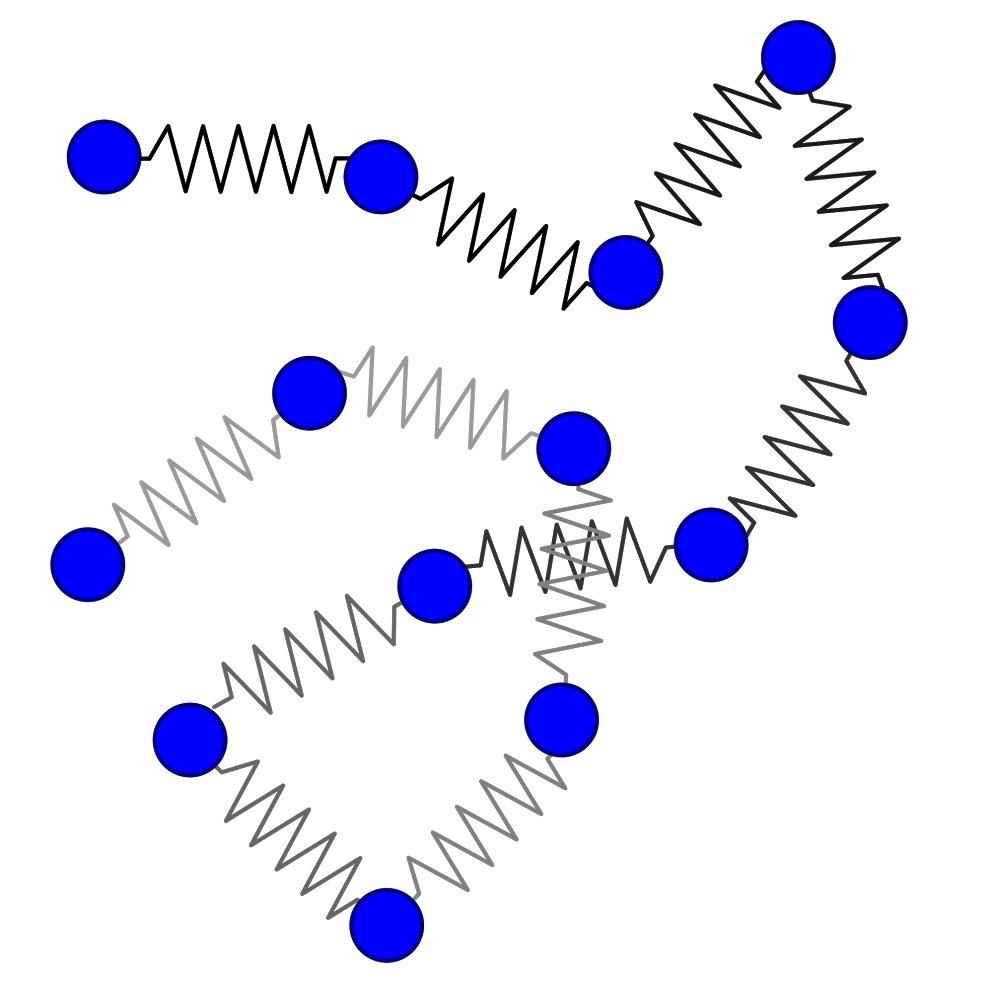
\includegraphics[width=0.3\textwidth]{beadspring.jpg}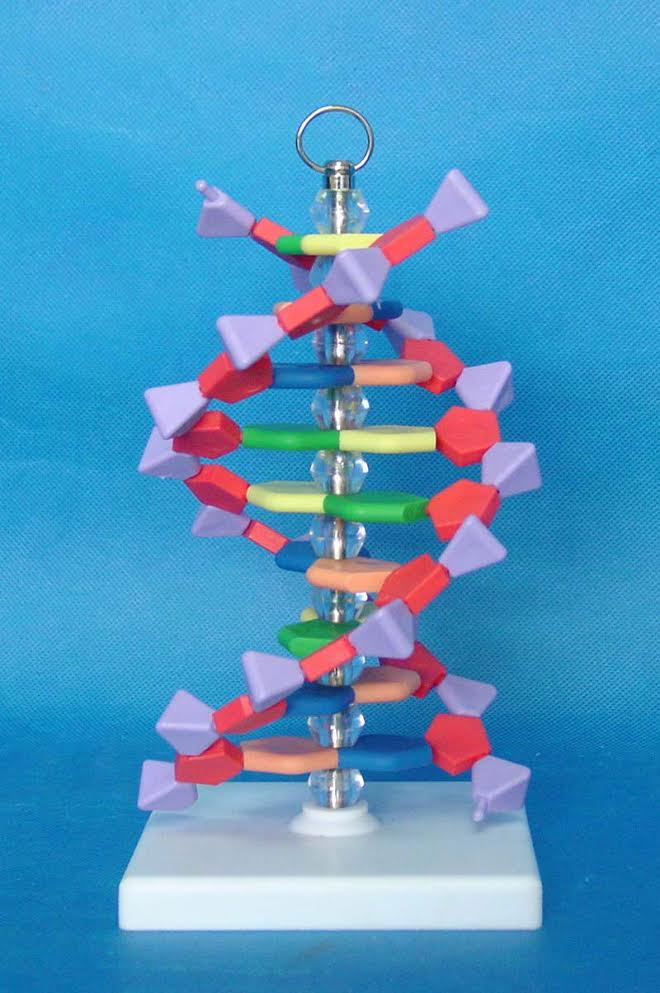
\includegraphics[width=0.21\textwidth]{coarsegraindnamodel.jpg}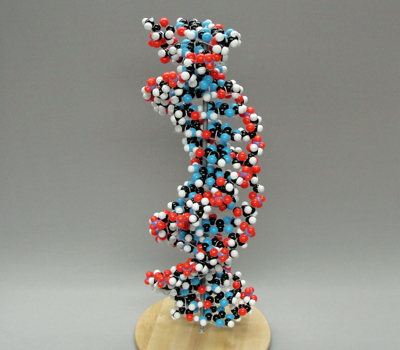
\includegraphics[width=0.36\textwidth]{fullatom.jpg}

\caption[Echelles de modèles]{Le modèle de Rouse \cite{Rouse1953} de niveau de détail faible est une simple succession de billes liées par des ressorts \cite{wikirouse}. Les modèles gros grains, rassemblant plusieurs atomes en une entité appelée grain présentent un niveau de détail intermédiaire \cite{coarsegrainmodna}. Le niveau de détail le plus fin est atteint par les modèles tout atomes \cite{fullatomdnamodel}.}
\label{echellemodeles}
\end{center}
\end{figure}



Le choix de l'échelle joue sur les comportements analysés. Un faible niveau de détail va faciliter l'obtention de lois de comportement générales car un ensemble statistique complet peut être investigué. En revanche si l'on souhaite regarder des propriétés particulières à certaines séquences d'ADN, un modèle à haute résolution est nécessaire. Une fois l'échelle choisie, il devient nécessaire d'employer un type de simulation adapté à cette échelle pour obtenir un modèle pertinent.


\subsection{Types de schémas numériques}

Il existe trois types de schémas numériques adaptés au problème de la translocation de polymères:
\begin{itemize}
\item Les méthodes de type Monte-Carlo
\item La Dynamique Moléculaire
\item Les simulations de type DFT (Density Functional Theory)

\end{itemize}

Chacun est adapté à certaines échelles et permet de vérifier des propriétés caractéristiques.\\

\subsubsection*{Les schémas numériques de type Monte-Carlo}  

Les méthodes de Monte-Carlo regroupent une large classe d'algorithmes de calculs qui se basent sur la répétition de tirages aléatoires pour obtenir des résultats numériques. Elles peuvent s'adapter à la résolution de tout problème probabiliste. La physique statistique des polymères donne un ensemble de loi probabilistes qui permettent d'intégrer des trajectoires de polymère par des algorithmes de type Monte-Carlo \cite{Verdier1962}. Typiquement, un maillage fin est réalisé dans le plan ou l'espace et un tirage de déplacements légers est imposé au parties constituante du polymère (voir figure \ref{montecarlotransloc}). Si l'énergie du nouveau tirage est inférieure à celle du précédent, il est conservé, sinon il est conservé avec une probabilité de $\exp(-\frac{\Delta H}{k_BT})$ ($H$ étant l'Hamiltonien du système) \cite{landau2009a}.

Ce type de modèle n'est efficace que pour un niveau de détails très faible et n'a été appliqué que pour des polymères linéaires simples. Les simulations de translocation de polymère par ces méthodes permettent de déterminer des comportements généraux (à travers des exposants critiques que nous définissons au \hyperref[taubiased]{chapitre 3}) \cite{Milchev2004,Kantor2004,2Luo2006,Tsuchiya2007,Dubbeldam2007}.



\begin{figure}[H]
\begin{center}
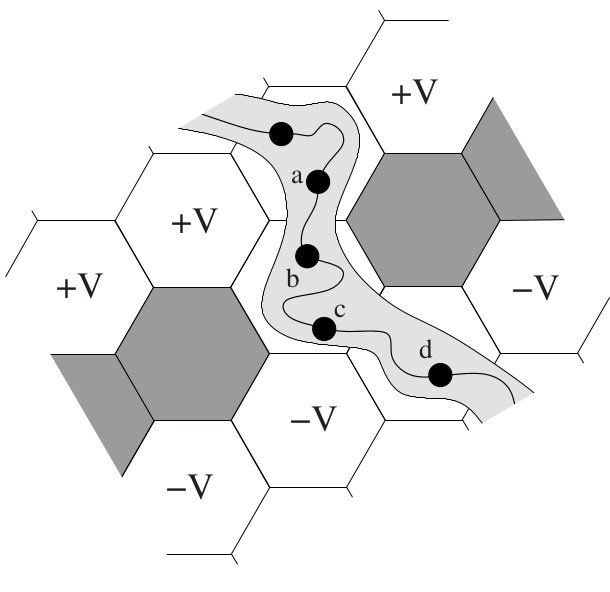
\includegraphics[width=0.6\textwidth]{montecarlotransloc.jpg}

\caption[Simulations de type Monte-Carlo]{Illustration d'un modèle de translocation de polymère résolu par une méthode de type Monte-Carlo \cite{these}. La translocation est biaisée par une différence de potentiel électrique, le polymère évolue dans un plan maillé par un réseau hexagonal.}
\label{montecarlotransloc}
\end{center}
\end{figure}





\subsubsection*{La Dynamique Moléculaire}

La dynamique moléculaire est une méthode de simulation numérique qui consiste en une intégration des équations du mouvement d'un système à N corps. Ces N corps (que l'on appellera grains) interagissent entre eux via des potentiels. Les équation de Newton sont ensuite résolues par un algorithme \cite{Verlet1967}. La force de la dynamique moléculaire est qu'elle peut s'adapter à toutes les échelles. En effet, si les N grains représentent des atomes, l'échelle tout atome est décrite, si ils représentent une chaîne d'oscillateurs couplés, un niveau de détail faible est modélisé et si ils représentent des molécules ou collections d'atomes, on obtient la description d'une échelle intermédiaire. Le problème de la translocation peut être abordé à n'importe quelle échelle grâce à la dynamique moléculaire.\\

Pour le niveau de détails le plus élevé, la première étape consiste à bien définir les interactions atomiques à l'aide d'un ensemble de champs de force moléculaires \cite{allen1987computer}. Ensuite il faut construire le système qui peut être, dans le cas du tout atome, identique aux conditions expérimentales \cite{Sathe2011,Farimani2014,Meunier2008,Chen2012,Kim2013,Postma2010,Jeong2013,Saha2012,Min2011,Aksimentiev2005,Aksimentiev2009,Heng2004,Heng2006}.
Bien que la précision soit alors très bonne, l'inconvénient de ce type de modèles est qu'il sont numériquement très gourmands en temps de calculs et les simulations sont donc limités à une échelle de temps réduite.

Des modèles simples, comme le modèle de Rouse par exemple peuvent également être utilisés pour déterminer des comportements généraux  \cite{Tian2003,Huopaniemi2006,Huopaniemi2007,Luo2008,Bhattacharya2009,Fyta2008,Luo2009,Ikonen2012}
(à l'instar des simulations de type Monte-Carlo). Nous allons nous même développer un modèle de polymère simple pour la translocation (voir \hyperref[porelargesimplepol]{chapitre 3}), avant d'augmenter le niveau de détails.

Il est possible de se situer entre ces deux échelles en utilisant des modèles dits gros grains. Les grains représentent alors un ensemble d'atomes. La translocation peut alors être abordée à l'échelle adaptée aux effets étudiés \cite{Forrey2007,Lansac2004,Ramachandran2011}. Nous utiliserons cette approche pour étudier la translocation d'un polymère structuré \hyperref[porelarge]{chapitre 3}.



\subsubsection*{La DFT}

La DFT n'est pas utilisée pour étudier la translocation a proprement parlé, elle est couplé à d'autres simulation afin de prédire les courants au cours de la translocation.




